
\subsection{Data Model}

\fmc{Modelo de Grafo - En general. Modelo PG escogido.}

\textcolor{gray}{Partes:
\begin{itemize}
    \item Justificación de por qué modelamos los datos con grafo y no de otra manera...
    \item Graph Database Model: Property graph model. Qué es un PG, por qué se elige...
    \begin{itemize}
        \item Simple/Easy to represent entities and their relationships with this data model.
        \item Good to represent dynamic data sources... relations constantly happening: modeled as edges of a graph (AMW2024 article)
        \item Good to represent evolving databases (AMW2024 article)
        \item (*) Direct way to model queries related to the search of fraud patterns: as graph patterns... query model (AMW2024 article) 
        \item Expressiveness of queries.
        \item Heuristics and indexing techniques that can be applied only if we operate in the domain of graphs: graph pattern matching and other optimizations... "translations of graphs into relations are unnatural and can not take advantage of graph-specific heuristics" (article \cite{PG-Graphs-at-a-time-GraphQL-QueryLanguage}: graph-at-a-time article).
    \end{itemize}
    \item Graph Database System: Neo4j. Otras opciones (relational database), por qué se elige...
    \item 
    \item Diferentes opciones
    \item Definir primero en general y luego definir la especificación en el caso del banco
\end{itemize}
References:
    \begin{itemize}
        \item PG: \cite{PG-angles2017foundations, PG-angles2018propertyGraphDatabaseModel, PG-Graphs-at-a-time-GraphQL-QueryLanguage, PG-exampleUsageSimeonovski}
        \item Graph Databases: \textcolor{blue}{\cite{GDB-angles2008survey, GDB-kumar2015graph}}
    \end{itemize}
}

\subsubsection*{Graph Database Model: Property Graph}

Informally, a property graph is a directed labeled multigraph with the special characteristic that each node or edge could maintain a set (possibly empty) of property-value pairs \cite{angles2018propertyGraphDatabaseModel}. In this graph, a node represents an entity, an edge a relationship between entities, and a property represents a specific feature of an entity or relationship. 
A more formally  (as defined in \cite{PG-exampleUsageSimeonovski}):

\begin{definition}
A property graph $G=(V,E, \lambda, \mu)$ is a directed labeled multigraph where $V$ is a set of nodes, $E \subseteq (V \times V)$ is a set of edges, $\lambda: V \cup E \rightarrow \Sigma$ is a function that labels nodes and edges with symbols of the alphabet $\Sigma$, and $\mu: (V \cup E) \times K \rightarrow S$ is a function that associates key-value properties, e.g., $(k,s)$ where $k \in K$ is the key and $s \in S$ is the string value, to nodes and edges.  
\end{definition}

\ad{Aqui estaría bien un ejemplo pequeño, dos nodos con un arco entre ellos y varias posibles propiedades, para que quede bien claro lo que es.}

\ad{añadir algo como lo siguiente: In the Graph Database community there several popular models of property graphs. Maybe the two most famous and used ones are \ldots 
los dos màs famosos con cita a algun sitio que diga que son los más famosos}

\ad{Muy importante: antes de explicar detalles específicos de Neo4j hay que explicar todo lo que es genérico de los property graphs y ponerlo aquí, fuera de la subsección de Neo4j}

\subsubsection*{Graph Database System: Neo4j}

Graph Databases: \textcolor{blue}{\cite{GDB-angles2008survey, GDB-kumar2015graph}}
% TODO: 
% - Poner definición 
% - Decir cuál elegimos: Neo4j y por qué

A graph database system is a system specifically designed for managing graph-like data following the basic principles of databases systems. 

\fmc{Describir el modelo de grafo escogido como data model: "Continuously evolving data graph"}

\newpage

\fmc{TODO: Describir el data model - como "Continuously evolving data graph" modelado como PG en el contexto de graph database. Poner todo como conjunto. Separación y razón de la separación del modelo en stable y volatile PGs.}
\textcolor{gray}{
Regarding the data model, the new nature of data requires a de facto new database paradigm
-continuously evolving databases- where data can be both stable and volatile. Even though
evolving databases can be implemented according to any approach, graph databases seem
especially well suited here [1, 2]. Indeed, the natural way to process evolving graphs as streams
of edges gives insights on how to proceed in order to maintain dynamic graph databases. Hence,
we consider that a suitable data model is a continuously evolving data graph, a graph having
persistent (stable) as well as non persistent (volatile) relations. Stable relations correspond
to edges occurring in standard graph databases while volatile relations are edges arriving indata streams during a set time interval. Once this time interval is over, the relations are not
longer valid so that there is no need to store them in the (stable) graph database. However,
when required -as for further legal or auditing purposes- timestamped occurrences of volatile
relations can be kept in a log file. Volatile relations induce subgraphs that exist only while the
relations are still valid. Without loss of generality, in this work we consider property graphs
(PG) [3, 4] as the basic reference data model. As an example, Figure 1a depicts part of a schema
of a PG database where stable relations correspond to the data that a bank typically gathers
on its issued cards, ATMs (Automated Teller Machines) network, etc. Volatile relations model
the interaction between cards and ATM entities}


\textcolor{blue}{In the context of our work we could see the data we are considering to be both static and streaming data, as we are considering a bank system application that contains all the information related to it on the cards, clients\dots, and that it is receiving the streaming of transactions that happens on it.
More specifically, the static data can be thinked of the classical bank database data, that is, the data a bank typically gathers on its issued cards, clients, accounts, ATMs\dots. Whereas as the streaming data we can consider the transactions the clients of the bank produce with their cards on ATMs, PoS\dots that reach the bank system.
Therefore, due to this nature of the data, we consider a \emph{continuously evolving database} paradigm, where data can be both stable and volatile. Even though 
evolving databases can be implemented according to any approach, graph databases seem especially well suited here \textcolor{blue}{\cite{angles2008survey, kumar2015graph}}. 
% TODO: PONER REFERENCIAS
% TODO: PONER + RAZONES?
}


The property graph data model consists of two sub property graphs: a stable and a volatile property graph. On the one hand, the stable is composed of the static part of the data that a bank typically gathers such as information about its clients, cards, ATMs (Automated Teller Machines). 
On the other hand, the volatile property graph models the transaction operations, which defines the most frequent and reiterative kind of interaction between entities of the data model.\\
The main difference and the main reason for this separation is the semantics with which we intentionally define each of the subgraphs: the stable will be understood like a fixed static bank database, whereas the volatile will be understood as the data model to define the transactions, as continuous interactions between the entities of the model, which will not be permanently saved, but instead, only for a certain window of time under the mission of detecting anomalous bank operations. Note that we will only model the transaction interaction in the volatile subgraph, only letting them occur here.
This separation will allow us to have a really simple and light property graph schema single-centered on the transactions with the minimal needed information (mostly identifiers of the entities a transaction links) and another, the stable, acting as a traditional bank database schema, from which to obtain the information details of the entities.

\fmc{Poner diferenciación entre Stable and Volatile PG. Por qué separamos el modelo en 2. Mostrar el PG completo conjunto.}

This property graph is a \emph{continuously evolving data graph}, which has a persistent (\emph{stable}) as well as non persistent (\emph{volatile}) relations. Stable relations correspond to edges occurring in standard graph databases while volatile relations are edges arriving in data streams during a set time interval. 

\fmc{Modelo de Grafo - Diseño de nuestro PG.}
\subsubsection*{Property Graph Data Model Design}

In what follows we describe the design of the Property Graph taken as our data model. Due to the confidential and private nature of bank data, it was impossible to find a real bank dataset nor a real bank data model. In this regard, we developed our own proposal of a bank database model taking as standard reference the \emph{Wisabi Bank Dataset}\footnote{https://www.kaggle.com/datasets/obinnaiheanachor/wisabi-bank-dataset}, which is a fictional banking dataset publicly available in the Kaggle platform. 

The proposed property graph data model is represented in Figure \ref{img:pg-complete}, consisting on both the stable and volatile property subgraphs merged. The details on both the stable and volatile property subgraphs are given next.

\begin{figure}[h]
  \centering
  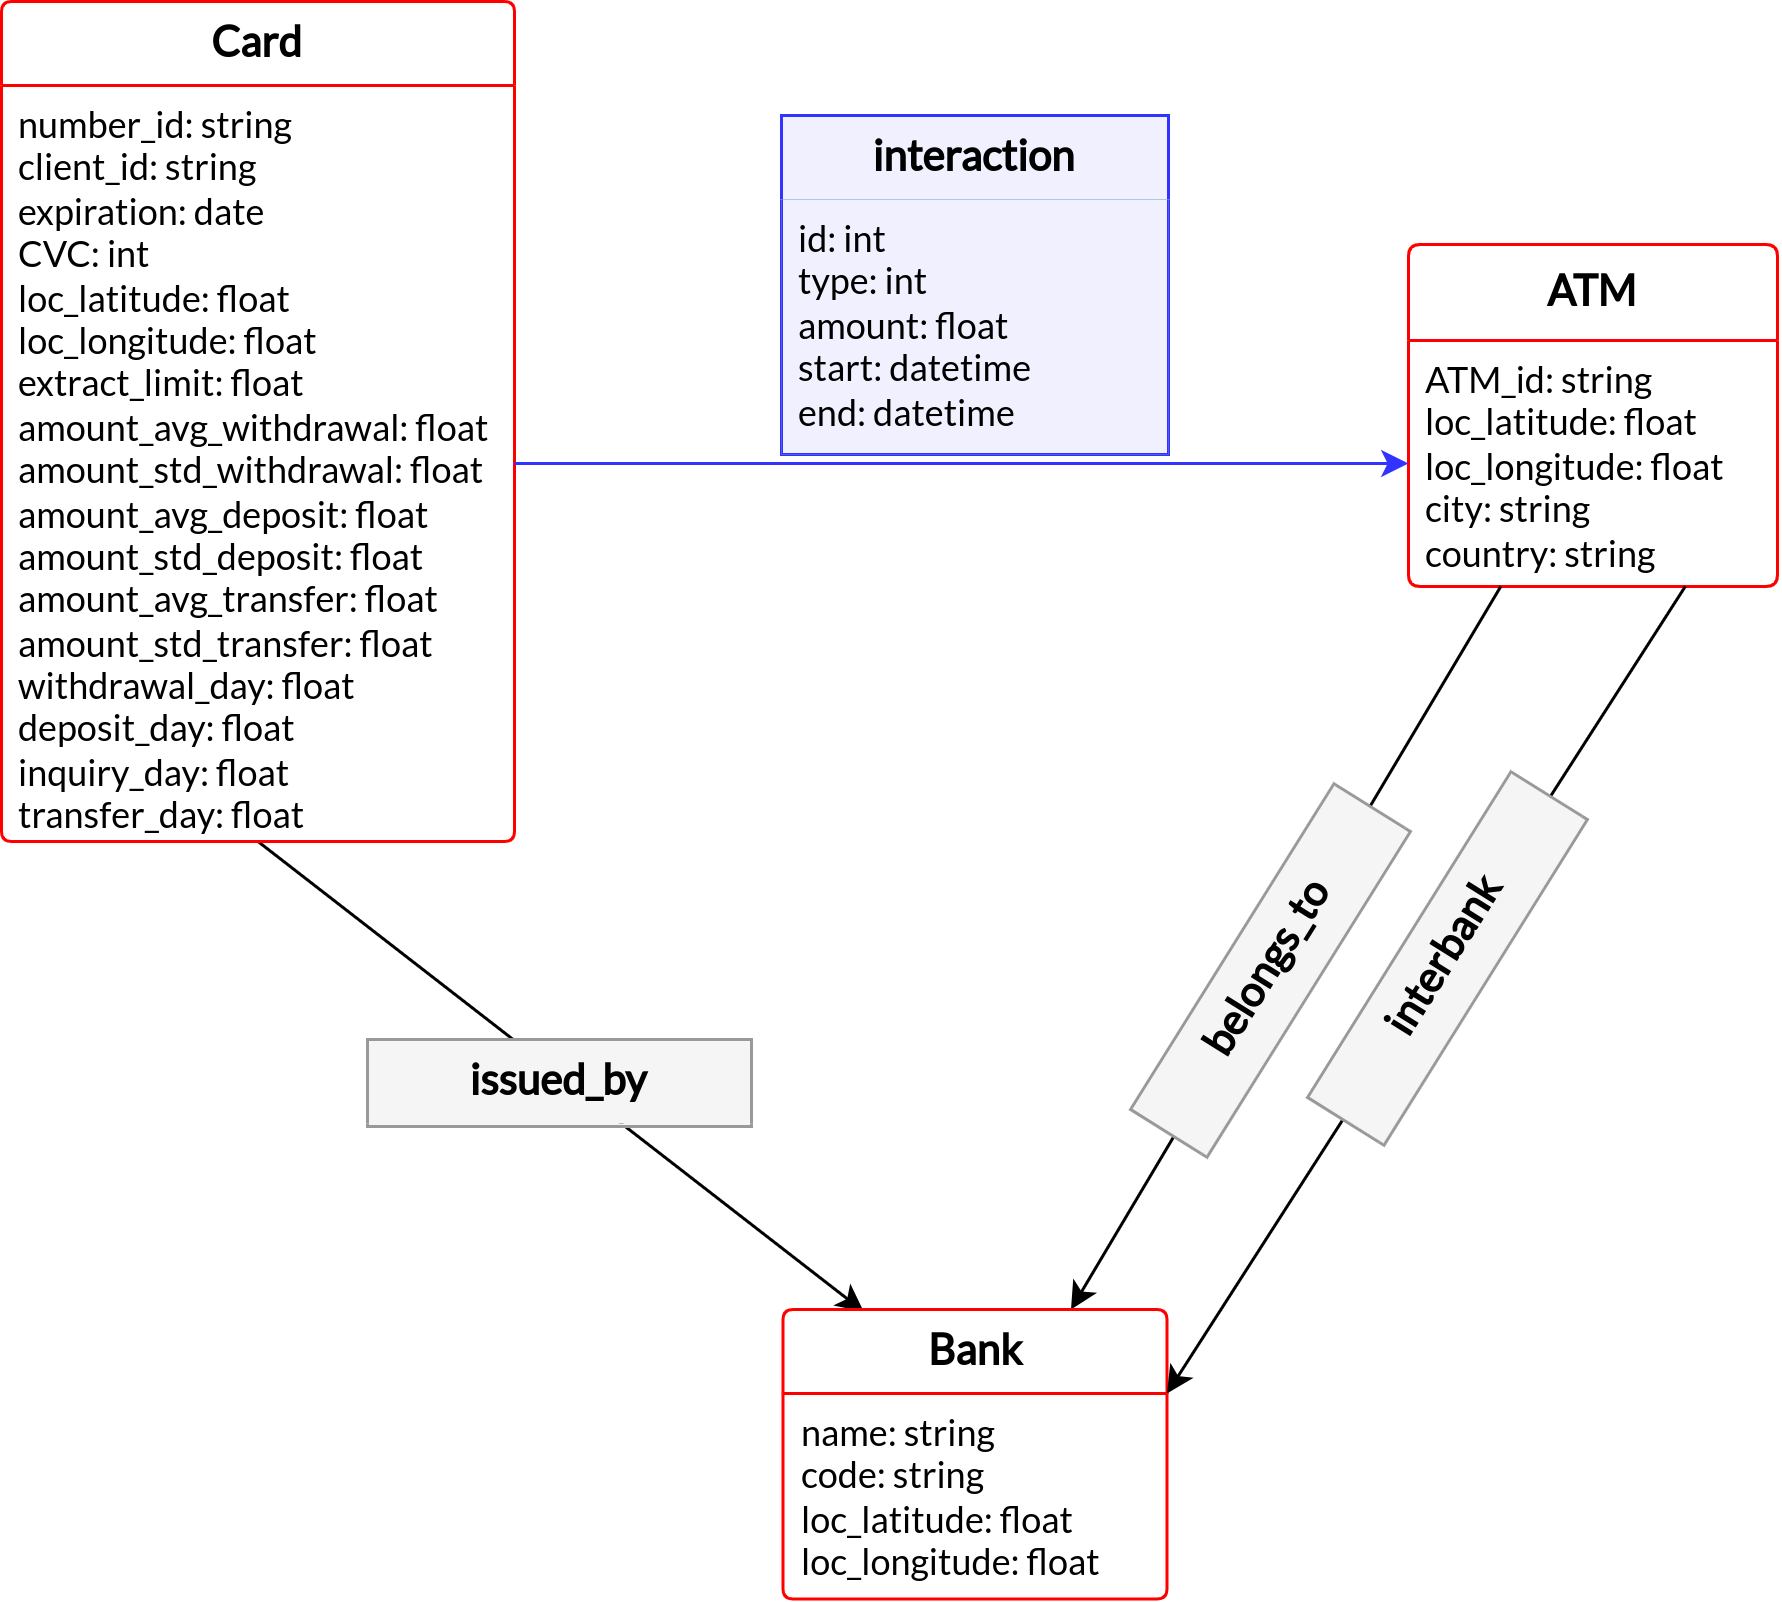
\includegraphics[scale = 0.7]{images/1-DataModel/PG-behavior-complete.png}
  \caption{Complete Property Graph Data Model}
  \label{img:pg-complete}
\end{figure}

\paragraph*{Stable Property Graph\\}\label{section:stable-pg}

Taking into account the reference dataset model, we designed a simplified version, as shown in Figure \ref{img:pg-stable-def}, with the focus on representing and modeling card-ATM interactions. On it, the defined entities, relations and properties modeling the bank database are reduced to the essential ones, which, we believe are enough to create a relevant and representative bank data model sufficient for the purposes of our work. Another option for the property graph data model representing a more common bank data model could be the one we defined in Figure \ref{img:pg-stable-big}, which intents to capture the data that a bank system database typically gathers. It consists of a more complete and possibly closer to reality data model, although unnecessarily complex for our objectives. 

\begin{figure}[h]
  \centering
  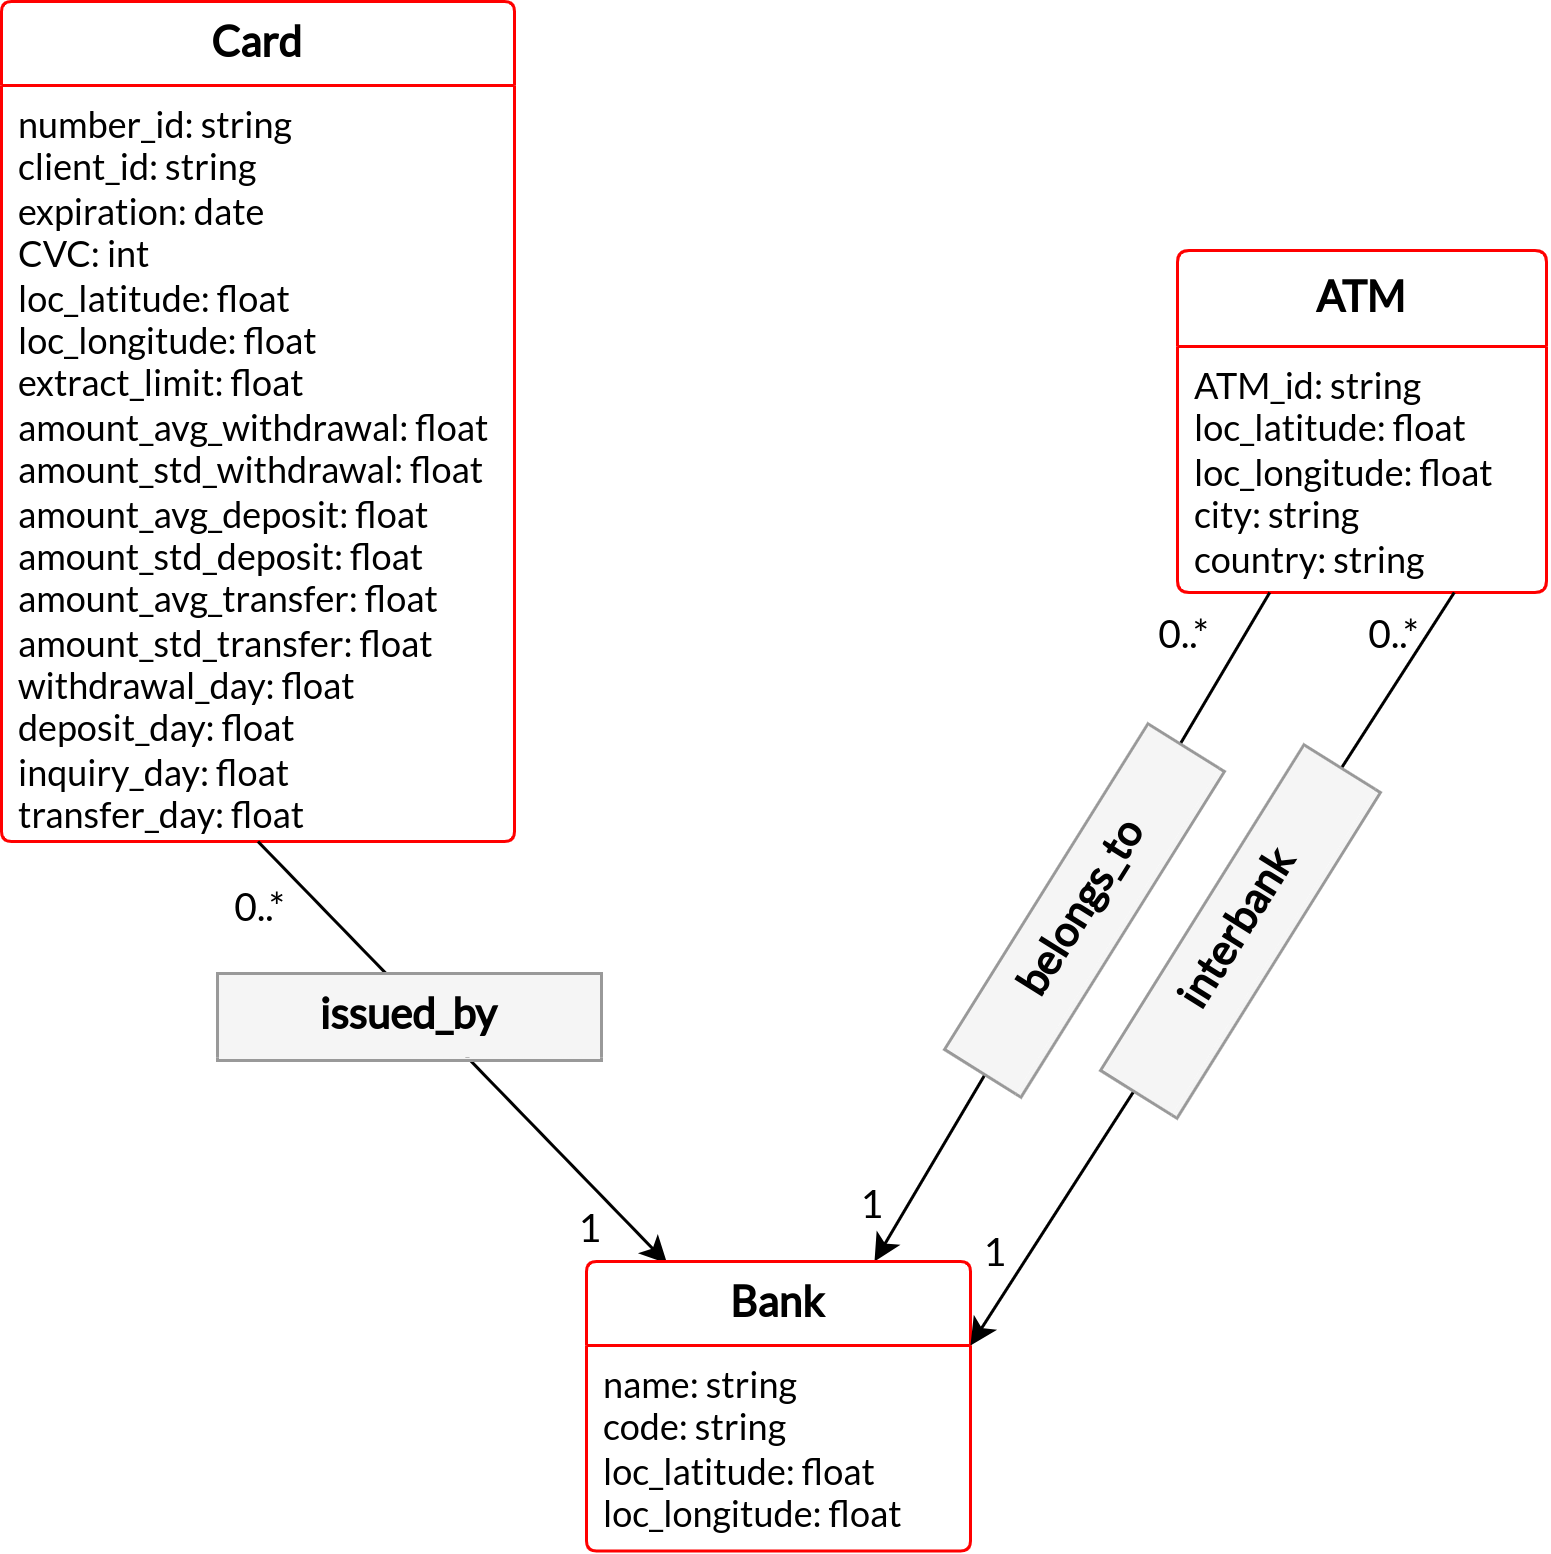
\includegraphics[scale = 0.7]{images/1-DataModel/PG-stable-behavior-cards.png}
  \caption{Stable Property Graph Data Model}
  \label{img:pg-stable-def}
\end{figure}

As a result, our definitive stable property graph model contains three node entities: Bank, Card and ATM, and three relations: \texttt{issued\_by} associating Card entities with the Bank entity, and \texttt{belongs\_to} and \texttt{interbank} associating the ATM entities with the Bank entity. 

% Bank
The Bank entity represents the bank we are considering in our system. Its properties consist
on the bank \emph{name}, its identifier \emph{code} and the location
of the bank headquarters, expressed in terms of \emph{latitude} and \emph{longitude}
coordinates, as seen in Table \ref{table:bank-node-properties}.
  
\begin{table}[H]
    \centering
      \begin{tabular}{|l|l|}
      \hline
      \textbf{Name}        & \textbf{Description and value}                                      \\ \hline
      \texttt{name}         & Bank name                                                 \\ \hline
      \texttt{code}         & Bank identifier code                                      \\ \hline
      \texttt{loc\_latitude}  & Bank headquarters GPS-location latitude                   \\ \hline
      \texttt{loc\_longitude} & Bank headquarters GPS-location longitude                  \\ \hline
      \end{tabular}
    \caption{Bank node properties}
    \label{table:bank-node-properties}
\end{table}

\fmc{Note that, from the beginning we were considering more than 1 bank entity. This lead to consider the creation of this entity, which now as only 1 bank is considered it may not be needed anymore, being able to reformulate and simplify the model. However, it is left since we considered it appropiate to be able to model the different kinds of ATMs a bank can have with different relation types instead of with different ATM types.}

The ATM entity represents the Automated Teller Machines (ATM) that either belong to the bank's network or that the bank can interact with.
% Potential possible generalization of the ATM entity to a POS entity
For the moment, this entity is understood as the classic ATM, however note that this entity could be potentially generalized to a Point Of Sale (POS) entity, allowing a more general kind of interactions apart from the current Card-ATM interaction, where also point-of-sale terminal transactions could be included apart from the ATM ones. 
\fmc{Also online / card not present (CNP) transactions?}
\fmc{El hecho de que se podría extender a la detección de otro tipo de fraude como el de PoS (Point of Sale) comentarlo también en otro apartado más visible y/o también el las conclusiones...}
We distinguish two different kinds of ATMs, depending on their relation with the bank:
\begin{itemize}
  \item Internal ATMs: ATMs owned and operated by the bank. They are fully integrated within the
  bank's network. Modeled with the \texttt{belongs\_to} relation.
  \item External ATMs: These ATMs, while not owned by the bank, are still accessible for the bank
  customers to perform transactions. Modeled with the \texttt{interbank} relation. 
\end{itemize}

Both types of ATMs are considered to be of the same type of ATM node. Their difference
is modeled as their relation with the bank instance: \texttt{belongs\_to} for the internal ATMs and \texttt{interbank} for the external ATMs.

\begin{table}[H]
    \centering
    \begin{tabular}{|l|l|}
    \hline
    \textbf{Property}        & \textbf{Description}                                      \\ \hline
    \texttt{ATM\_id}      & ATM unique identifier                             \\ \hline
    \texttt{loc\_latitude}  & ATM GPS-location latitude           \\ \hline
    \texttt{loc\_longitude} & ATM GPS-location longitude          \\ \hline
    \texttt{city}         & ATM city location                         \\ \hline
    \texttt{country}      & ATM country location                       \\ \hline
    \end{tabular}
    \caption{ATM node properties}
    \label{table:atm-node-properties}
\end{table}

The ATM node type properties consist on the ATM unique identifier \emph{ATM\_id}, its location, expressed in terms of \emph{latitude} and \emph{longitude} coordinates, and the \emph{city} and 
\emph{country} in which it is located, as seen in Table \ref{table:atm-node-properties}.
Note that the last two properties are somehow redundant, considering that location coordinates
are already included. In any case both properties are maintained since their inclusion provides a more explicit and direct description of the location of the ATMs, which will be of special interest for some of the card anomalous patterns that will be considered.\\

Finally, the Card node type represents the cards of the clients in the bank system. The Card node type properties, as depicted in Table
\ref{table:card-node-properties}, consist on the card unique 
identifier \emph{number\_id}, the associated client unique identifier \emph{client\_id}, the card validity expiration date \emph{expiration}, the Card Verification Code, \emph{CVC}, the coordinates of the associated client habitual residence address \emph{loc\_latitude} and 
\emph{loc\_longitude} and the \emph{extract\_limit} property, which represents the limit on the amount of money it can be extracted with the card on a single withdrawal, related with the the amount of money a person owns. These last two properties are of special interest for some future card fraud patterns to be considered. In the first case related with interactions far from the client's habitual residence address and in the second with unusually frequent or very high expenses interactions.

Finally it contains the properties related with the \emph{behavior} of the client, representing the usual comportment of a client in regard with its ATM usage: \emph{amount\_avg\_withdrawal}, \emph{amount\_std\_withdrawal}, \emph{amount\_avg\_deposit}, 
\emph{amount\_std\_deposit}, \emph{amount\_avg\_transfer},  \emph{amount\_std\_transfer}, \emph{withdrawal\_day}, \emph{deposit\_day}, \emph{transfer\_day} and \emph{inquiry\_day}.
They are metrics representing the behavior of the owner of the Card, and they are included as properties as we think they could be of interest to allow the detection of some kinds of anomalies related with anomalous client's behavior in the future.

\begin{table}[H]
    \centering
    \begin{tabular}{|l|l|}
    \hline
    \textbf{Name}        & \textbf{Description and value}                                          \\ \hline
    \texttt{number\_id}   & Card unique identifier                               \\ \hline
    \texttt{client\_id}   & Client unique identifier                               \\ \hline
    \texttt{expiration}   & Card validity expiration date                      \\ \hline
    \texttt{CVC}          & Card Verification Code                                      \\ \hline
    \texttt{extract\_limit} & Card money amount extraction limit    \\ \hline
    \texttt{loc\_latitude}  & Client's habitual address GPS-location latitude                         \\ \hline
    \texttt{loc\_longitude} & Client's habitual address GPS-location longitude                        \\ \hline
    \end{tabular}
    \caption{Card node properties}
    \label{table:card-node-properties}
\end{table}

The client is completely anonymized in the system (no name, surname, age, or any other confidential details) by using only a \emph{client\_id}. Currently, \emph{client\_id} is included in the Card node type for completeness. However, it could be omitted for simplicity, as we assume a one-to-one relationship between card and client for the purposes of our work -- each card is uniquely associated with a single client, and each client holds only one card. Thus, the \emph{client\_id} is not essential at this stage but is retained in case the database model is expanded to support clients with multiple cards or cards shared among different clients.

\begin{figure}[h]
  \centering
  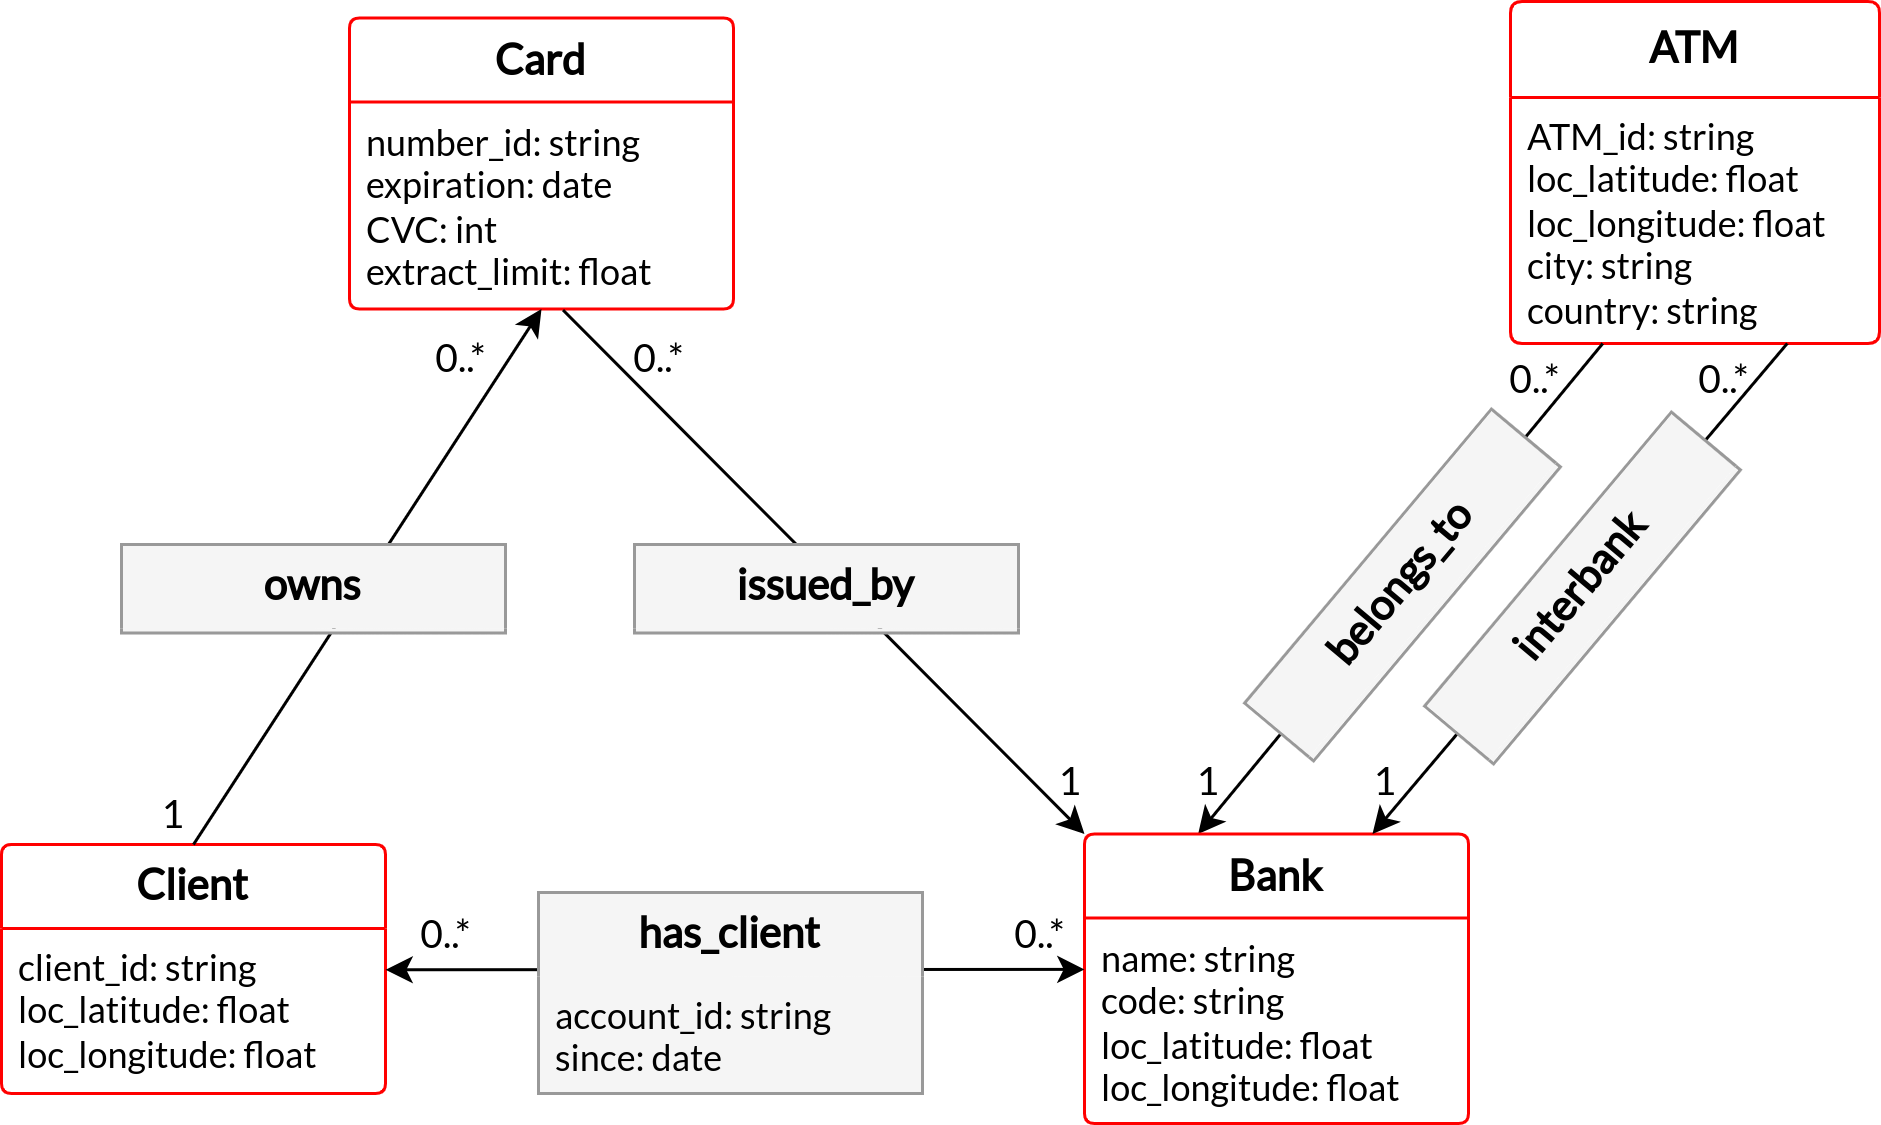
\includegraphics[scale = 0.7]{images/1-DataModel/PG-stable-edit-cardinal.png}
  \caption{Alternative - Complex Stable Property Graph Data Model}
  \label{img:pg-stable-big}
\end{figure}

\fmc{Describir el modelo más complejo? / el inicial?}

The more complex alternative model, shown in Figure \ref{img:pg-stable-big}, contains four entities: Bank, ATM, Client and Card with their respective properties, and the corresponding relationships between them. The relations are: a directed relationship from Client to Card \texttt{owns} representing that a client can own multiple credit cards and that a card is owned by a unique client, then a bidirectional relation \texttt{has\_client} between Client and Bank; representing bank accounts of the clients in the bank. The relation between Card and Bank to represent that a card is \texttt{issued\_by} the bank, and that the bank can have multiple cards issued. Finally, the relations \texttt{belongs\_to} and \texttt{interbank} between the ATM and Bank entities, representing the two different kinds of ATMs depending on their relation with the bank; those ATMs owned and operated by the bank and those that, while not owned by the bank, are still accessible for the bank customers to perform transactions.

This model allows a more elaborated representation of what a bank system database is. As it can be seen it represents clients as an independent entity from the Card entity, and it also allows to represent bank accounts through the relation between the Client and Bank entities. 

\fmc{Quitar esto ya?}
\ad{Sí, todo lo que no te sirva quítalo o comentalo ya, guarda el texto por si te puede llegar a hacer falta pero ya ve avanzando en la versión más definitiva del documento.}
\textcolor{gray}{
On the final version of the model, we decided to remove the Client entity and to merge it inside the Card entity. For this, all the Client properties were included in the Card entity. In the complete data model schema (Figure \ref{img:pg-stable-big}) the Client entity was defined with three properties: the identifier of the client and the GPS coordinates representing the usual residence of the client. This change is done while preserving the restriction of a Card belonging to a unique client the same way it was previously done with the relation between Card and Client \texttt{owns} in the complete schema, which now is therefore removed.} \\
% Account relation removed
\textcolor{gray}{
Another derived consequence of this simplification is the removal of the other relation that the Client entity had with other entities: the \texttt{has\_client} relation between Client and Bank, which was made with the intention of representing the bank accounts between clients and banks. Maintaining a bank account would imply having to consistently update the bank account state after each transaction of a client, complicating the model. Nevertheless, we eliminate the bank account relation, since its removal is considered negligible and at the same time helpful for the simplification of the model needed for the purposes of our work. % Properties included with the purpose of detecting frauds 
However, for the sake of completeness the property \textit{extract\_limit} is introduced in the Card entity, representing a money amount limit a person can extract, which will be related with the amount of money a person owns. This will allow the detection of anomalies related with frequent or very high expenses. Other properties that are included with the purpose of allowing the detection of some other kinds of anomalies are the GPS coordinates and the client's \emph{behavior} properties. The GPS coordinates are added in the ATM and Card entities, in the first case referring to the geolocation of each specific ATM and in the last case referring to each specific client address geolocation. The client's \emph{behavior} properties are added in the Card entity. They are metrics representing the behavior of the owner of the Card, and they are included as properties as we think they could be of interest to allow the detection of some kinds of anomalies in the future.}


\paragraph*{Volatile Property Graph\\}\label{section:volatile-pg}

The volatile property graph consists on an abstraction of the property graph model to describe the interactions between the cards and the ATMs in the bank system (see it on Figure \ref{img:pg-volatile}). These interactions are going to be continuously occurring and arriving to our system as data stream.

This property graph is a subgraph of the original bank property graph model. It contains the Card and ATM entities with the minimal information needed to identify them -- \emph{number\_id} and \emph{ATM\_id}, Card and ATM identifiers, respectively -- between which the interaction occurs, along with additional details related to the interaction. Those identifiers are enough to be able to recover, if needed, the whole information about the specific Card or ATM entity in the stable property graph.

\begin{figure}[h]
    \centering
    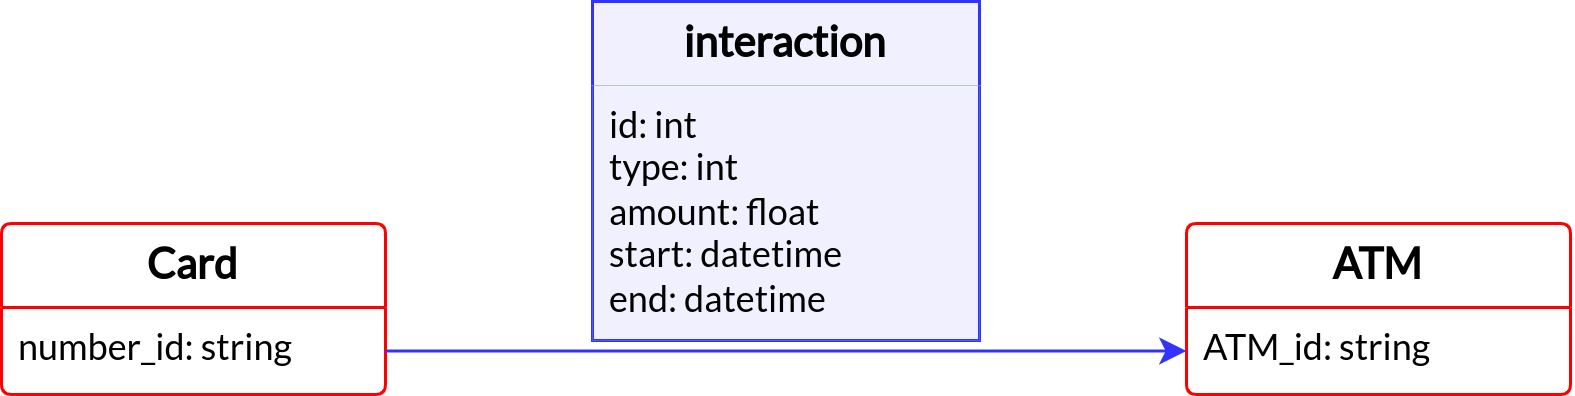
\includegraphics[scale = 0.8]{images/1-DataModel/schema-volatile.png}
    \caption{Volatile Property Graph Data Model}
    \label{img:pg-volatile}
\end{figure}

Finally, it contains the \emph{interaction} relationship between the Card and the ATM nodes. The \emph{interaction} relation contains as properties: \emph{id} as the interaction unique identifier, \emph{type} which describes the type of the interaction (withdrawal, deposit, balance inquiry or transfer), \emph{amount} describing the amount of money involved in the interaction in the local currency considered, and finally, \emph{start} and \emph{end} which define the interaction \emph{datetime} start and end moments, respectively. 

\fmc{TODO: Poner tabla de propiedades de la relacion interaction como con las propiedades de las entities: Bank, Card y ATM}

\fmc{TODO: Poner aqui lo de interaction start y end, la diferenciación y el por qué. En lugar de hacerlo en el apartado de la generación de transacciones}

\begin{comment}
\begin{itemize}
  \item[-] transaction\_id: Unique identifier for each transaction in the database.
  \item[-] transaction\_start: Datetime when the transaction started. Format: DD/MM/YYYY HH:MM (ex. 1/1/2022 4:50).
  \item[-] transaction\_end: Datetime when the transaction was completed. Format: DD/MM/YYYY HH:MM (ex. 1/1/2022 4:54).
  \item[-] transaction\_amount: Amount of money involved in the transaction.
\end{itemize}

\begin{figure}[H]
    \centering
    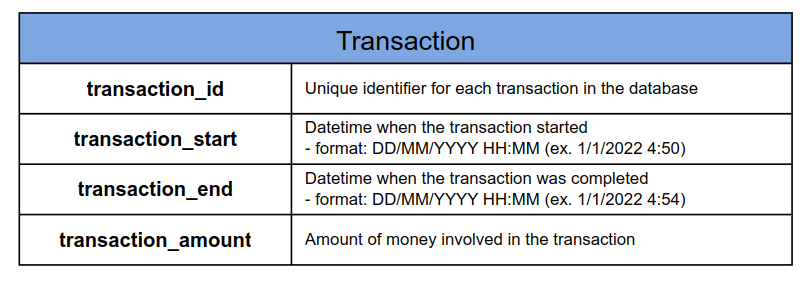
\includegraphics[scale = 0.40]{images/transaction.png}
    \caption{Transaction relation attributes}
    \label{img:pg-stable}
\end{figure}

\end{comment}

\subsection{Generation of the Synthetic Dataset}

As previously mentioned, given the confidential and private nature of bank data, it was not possible to find any real bank dataset. In this regard, we had to design and generate our own synthetic stable property graph bank database and stream of synthetic transactions. 

\ad{Hay que explicar porqué no servía y citar los artículos originales.}

In what follows we explain all the work related with the generation of the synthetic dataset that was used to build the stable graph databases and interaction data streams for the proof of concept of our system.

\subsubsection*{Reference Dataset: Wisabi Bank Dataset}

For the generation of our synthetic database and stream of transactions we considered to take as a standard data reference the \emph{Wisabi Bank Dataset}\footnote{\href{https://www.kaggle.com/datasets/obinnaiheanachor/wisabi-bank-dataset}{Wisabi bank dataset on kaggle}}, which is a fictional banking dataset publicly available in the Kaggle platform. We used it as a first base to do general customisable programs for the generation of synthetic bank datasets and streams of transactions.

The interest to use this bank dataset as a base was mainly because it is large enough and it also contained a card-ATM transactions dataset. Additionally, it provides good heterogeneity on the different kind of transactions: withdrawals, deposits, balance inquiries and transfers. 
The details of the \emph{Wisabi Bank Dataset} are summarized next.
 
\begin{itemize}
    \item 8819 customers.
    \item 50 different ATM locations.
    \item 2143838 card-ATM transactions records of the different customers during a full year (2022) on five different states of Nigeria (Federal Capital Territory, Lagos, Kano, Enugu and Rivers State).
\end{itemize}

The dataset consists on ten \emph{csv} tables each with different information which is summarized on Table~\ref{table:wisabi-summary}.

\begin{table}[H]
\centering
\begin{tabular}{|l|l|}
\hline
\textbf{Name of the Table}                                                                                               & \textbf{Description}                                              \\ \hline
enugu\_transactions                                                                                 & Transactions of Enugu state (350251 transactions)                     \\ \hline
fct\_transactions                                                                                   & Transactions of Federal Capital Territory state \\ & (159652 transactions) \\ \hline
kano\_transactions                                                                                  & Transactions of Kano state (458764 transactions)                      \\ \hline
lagos\_transactions                                                                                 & Transactions of Lagos state (755073 transactions)                     \\ \hline
rivers\_transactions                                                                                & Transactions of Rivers state (420098 transactions)                    \\ \hline
customers\_lookup                                                                                   & Data of the different cardholders (8819 cardholders)                 \\ \hline
atm\_location\_lookup                                                                               & Data of the different ATM locations (50 ATMs)                 \\ \hline
\begin{tabular}[c]{@{}l@{}}calendar\_lookup, hour\_lookup,\\ transaction\_type\_lookup\end{tabular} & Complementary data of the previous tables                \\ \hline
\end{tabular}
\caption{Wisabi Bank Dataset Tables Summary}
\label{table:wisabi-summary}
\end{table}

The main usage that we did of this dataset was the obtention of a geographical distribution of the ATM locations and the construction of a card/client \emph{behavior} based on the ATM-card transactions records provided.

In particular, as for the data model, we divide the creation of the synthetic dataset in two. On the one hand the creation of the stable bank dataset and on the other hand the creation of the synthetic and anomalous transactions dataset that will conform the data stream reaching our system.

\subsubsection*{Stable Bank Dataset Generation}

\paragraph{Bank dataset generator: \texttt{bankDataGenerator.py}\\\\}\label{bankDataGenerator}
To do the generation of a stable bank dataset we developed the Python program \texttt{bankDataGenerator.py}. 
To use it we only need to enter the bank properties' values, and the number of the bank ATMs (internal and external) \texttt{n} and Cards \texttt{m} to be generated. With this program we can generate the \emph{csv} files which define the bank dataset. A directory named \texttt{csv} will be created with the following files: 

\begin{itemize}
    \item \texttt{bank.csv}: bank entity.
    \item \texttt{atm.csv}: ATM entities.
    \item \texttt{card.csv}: card entities.
    \item \texttt{atm-bank-external.csv}: external ATM-bank relations.
    \item \texttt{atm-bank-internal.csv}: internal ATM-bank relations.
    \item \texttt{card-bank.csv}: card-bank relations.
\end{itemize}
To use it:
% How to use the bankDataGenerator

\begin{enumerate}
    \item Ensure to have a \texttt{wisabi} named directory with the \emph{csv} files downloaded from the \emph{Wisabi Bank Dataset} on Kaggle.\footnote{\href{https://www.kaggle.com/datasets/obinnaiheanachor/wisabi-bank-dataset}{Wisabi bank dataset on kaggle}}.
    \item Ensure to have the \texttt{behavior.csv} file or run \texttt{\$> python3 behavior.py} to create it.
    \item Run \texttt{\$> python3 bankDataGenerator.py} -- \textcolor{gray}{Run with Python3.6 version or higher} -- and introduce:
    \begin{enumerate}
        \item Bank properties' values.
        \item $n = |ATM|$, internal and external.
        \item $m = |Cards|$.
    \end{enumerate}
\end{enumerate}

In what follows we give the details on the generation of the instances of our static dataset entities.

\fmc{Esto ponerlo en otr sitio:}
\textcolor{gray}{
For simplicity and to do it in a more stepwise manner, we are going to first create all the CSV data tables for the nodes and for the relations in the corresponding format and then we will populate the Neo4j GDB with them.}

\paragraph{Bank entity: \texttt{bank.csv}\\\\}

Since a unique bank instance is considered, the values of the properties of the bank node are manually assigned, leaving them completely customisable (see an example on \ref{csv:bank}).

\begin{center}
\lstset{style=csvStyle}
\begin{lstlisting}[caption={Example of a bank.csv}, label={csv:bank}]
                    name,code,loc_latitude,loc_longitude
                    Niger Bank,NIGER,6.478685,3.368442
\end{lstlisting}
\end{center}

\paragraph{ATM entity: \texttt{atm.csv}\\\\}

We generate $\texttt{n = n\_internal + n\_external}$ ATMs (\texttt{n\_internal} ATMs owned by the bank and \texttt{n\_external} external ATMs not owned by the bank, but still accessible
for the bank customers to perform transactions). See an example in \ref{csv:atm}.

\begin{itemize}
    \item \textbf{ATM identifier}: \emph{ATM\_id}. It is assigned a different code depending on the ATM internal or external relation of the ATM with the bank: 
        \[
        \emph{ATM\_id} =
        \begin{cases} 
        bank\_code \text{-} i & 0 \leq i < \texttt{n\_internal } \text{if internal ATM}  \\
        EXT \text{-} i & 0 \leq i < \texttt{n\_external } \text{if external ATM}
        \end{cases}
        \]
    \item \textbf{Geographical properties}: \emph{city}, \emph{country}, \emph{loc\_latitude}         and \emph{loc\_longitude}. 
        They are assigned following the geographical distribution of the locations of the ATMs in the \emph{Wisabi Bank Dataset}. 
        On this dataset there are 50 ATMs locations distributed along Nigerian cities. 
        Note that for each of these ATMs locations, there can be more than one ATM.
        However, this is not taken into account and only one ATM per location is assumed for the 
        distribution. This distribution of the ATMs matches the relevance of the location in terms of its population, since the number of ATM locations is larger in the most populated 
        Nigerian cities (30\% of the ATM locations are in the city of Lagos, then the 20\% in Kano...).
        
        \fmc{Put plot of the ATMs geographical distribution?}
        \ad{Si, estaria bien, un ejemplo}
        
        With this, we assign each of the \texttt{n} ATMs \emph{city} and \emph{country} properties a random location/city from the \emph{Wisabi Bank Dataset}, and we then produce random geolocation coordinates inside the bounding box of the city location to set as the \emph{loc\_latitude} and \emph{loc\_longitude} properties of the ATM. \\
\end{itemize}

\begin{center}
\lstset{style=csvStyle}
\begin{lstlisting}[caption={Example of atm.csv}, label={csv:atm}]
                ATM_id,loc_latitude,loc_longitude,city,country
                NIGER-0,12.124651,8.543515,Kano,Nigeria
                NIGER-1,12.148756,8.481764,Kano,Nigeria
                EXT-0,8.941474,7.526291,Abuja,Nigeria
                EXT-1,4.816251,7.010188,Port Harcourt,Nigeria
\end{lstlisting}
\end{center}

\paragraph{Card entity: \texttt{card.csv}\\\\}

We generate a total of \texttt{m} cards that the bank manages. For each of them the assignment of the different properties is done as explained next. An example of a Card data item can be seen in \ref{csv:card}.

\begin{itemize}
\item \textbf{Card and client identifiers}:

\[
\begin{cases} 
number\_id = \text{c-}bank\_code\text{-}i \\
client\_id = i 
\end{cases}
0 \leq i < \texttt{m}
\]

\item \textbf{\emph{expiration} and \emph{CVC} properties}: they are not relevant, could be empty value properties indeed or a same toy value for all the cards. The same values are given for all the cards: $expiration = \text{2050-01-17}$, $CVC = 999$.

\item \textbf{Client's habitual address location (\emph{loc\_latitude}, \emph{loc\_longitude})}: two possible options were designed to define the client habitual residence address. In both 
cases they are random 
coordinates drawn from a bounding box of a location/city. The difference is on how the selection of the location/city is done:

  \begin{enumerate}
      \item \textbf{Wisabi customers selection}: take the city/location of the usual ATM of a random selected \emph{Wisabi} database customer. Note that in the \emph{Wisabi Bank Dataset} customers contain an identifier
      of their usual ATM, more in particular, the dataset is designed in such a way that customers
      only perform operations in the same ATM.
      With this approach, we maintain the geographical distribution of the \emph{Wisabi} customers.
      \item \textbf{Generated ATMs selection}: take the city/location of a random ATM of the \texttt{n} generated ATMs. This method is the one utilized so far.
  \end{enumerate}

\item \textbf{\emph{Behavior} properties}: these are properties of special interest both when performing the 
generation of the synthetic transactions of each of the cards and also for the detection of future possible fraud patterns. The defined \emph{behavior} properties are shown in Table \ref{table:behavior-properties}. They refer about metrics related with four different types of operations: withdrawal, deposit, balance inquiry and transaction. These operations will be the ones that, as in the base dataset, we will also consider that a customer can perform when we generate our synthetic transaction dataset.

\begin{table}[H]
    \centering
    \begin{tabular}{|l|l|}
        \hline
        \textbf{Behavior Property} & \textbf{Description} \\ 
        \hline
        $\mathsf{amount\_avg\_withdrawal}$ & Withdrawal amount mean\\ 
        \hline
        $\mathsf{amount\_std\_withdrawal}$ & Withdrawal amount standard deviation \\ 
        \hline
        $\mathsf{amount\_avg\_deposit}$ & Deposit amount mean \\ 
        \hline
        $\mathsf{amount\_std\_deposit}$ & Deposit amount standard deviation\\ 
        \hline
        $\mathsf{amount\_avg\_transfer}$ & Transfer amount mean \\ 
        \hline
        $\mathsf{amount\_std\_transfer}$ & Transfer amount standard deviation \\ 
        \hline
        $\mathsf{withdrawal\_day}$ & Average number of withdrawal operations per day \\ 
        \hline
        $\mathsf{deposit\_day}$ & Average number of deposit operations per day \\ 
        \hline
        $\mathsf{transfer\_day}$ & Average number of transfer operations per day \\ 
        \hline
        $\mathsf{inquiry\_day}$ & Average number of inquiry operations per day \\ 
        \hline
    \end{tabular}
    \caption{\emph{Behavior} properties}
    \label{table:behavior-properties}
\end{table}


The behavior properties' values are assigned to each of the cards by taking a random behavior \emph{row} from the \texttt{behavior.csv} file. This \texttt{behavior.csv} contains the gathered behavior metrics of each of the customers of the \emph{Wisabi Bank Dataset}. It was generated by using the Python program \texttt{behavior.py}. This program creates the behavior of each of the original customers of the \emph{Wisabi Bank Dataset} by doing a summary of all its transaction records on this base dataset.

Another possible way to assign the \emph{behavior} parameters could be the assignation
of the same behavior to all of the card instances. However, this method will provide less variability in
the generation of the synthetic transactions than the aforementioned method. 
Nevertheless, other taylored generation methods to generate different \emph{behavior} for 
each the cards could also be considered to similarly obtain this
variability.

\item \textbf{Card money amount extraction limit property}: \emph{extract\_limit}. We set it up by setting an upper bound based on the \emph{amount\_avg\_withdrawal} behavior metric of the card. Other possible ways could be chosen for assigning a value to this property.
    $$extract\_limit: amount\_avg\_withdrawal * 5$$
\end{itemize}

\begin{center}
\lstset{style=csvStyle}
\begin{lstlisting}[caption={Example of card.csv (Part 1)}, label={csv:card}]
    number_id,client_id,expiration,CVC,loc_latitude,loc_longitude,extract_limit
    c-NIGER-0,0,2050-01-17,999,8.92926,7.398833,121590.9
\end{lstlisting}
\end{center}

\begin{center}
\lstset{style=csvStyle}
\begin{lstlisting}[caption={Example of card.csv (Part 2)}]
        amount_avg_withdrawal,amount_std_withdrawal,withdrawal_day
        24318.18,28174.96,0.2411
\end{lstlisting}
\end{center}

\begin{center}
\lstset{style=csvStyle}
\begin{lstlisting}[caption={Example of card.csv (Part 3)}]
        amount_avg_deposit,amount_std_deposit,deposit_day,inquiry_day
        11500.0,5889.33,0.0548,0.0493
\end{lstlisting}
\end{center}

\begin{center}
\lstset{style=csvStyle}
\begin{lstlisting}[caption={Example of card.csv (Part 4)}]
        amount_avg_transfer,amount_std_transfer,transfer_day
        21448.28,20500.15,0.0795
\end{lstlisting}
\end{center}

\paragraph{ATM-Bank \texttt{interbank} relation: \texttt{atm-bank-external.csv}\\\\}

To represent the \texttt{interbank} relations between the bank and the external ATMs. Taking the unique ids of each of the related entities, the bank \emph{code} and the \emph{ATM\_id}. Example on \ref{csv:atm-bank-external}.

\begin{center}
\lstset{style=csvStyle}
\begin{lstlisting}[caption={Example of a atm-bank-external.csv}, label={csv:atm-bank-external}]
                                code,ATM_id
                                NIGER,EXT-0
                                NIGER,EXT-1
\end{lstlisting}
\end{center}

\paragraph{ATM-Bank \texttt{belongs\_to} relation:\texttt{atm-bank-internal.csv}\\\\}

To represent \texttt{belongs\_to} relations between the bank and the internal ATMs. Taking the unique ids of each of the related entities, the bank \emph{code} and the \emph{ATM\_id}. Example on \ref{csv:atm-bank-internal}.

\begin{center}
\lstset{style=csvStyle}
\begin{lstlisting}[caption={Example of a atm-bank-internal.csv}, label={csv:atm-bank-internal}]
                                code,ATM_id
                                NIGER,NIGER-0
                                NIGER,NIGER-1
                                NIGER,NIGER-2
\end{lstlisting}
\end{center}

\paragraph{Card-Bank \texttt{issued\_by} relation: \texttt{card-bank.csv}\\\\}

To represent the \texttt{issued\_by} relations between the bank and the card entities. Taking the unique ids of each of the related entities, the bank \emph{code} and the Card id: \emph{number\_id}. Example on \ref{csv:card-bank}.

\begin{center}
\lstset{style=csvStyle}
\begin{lstlisting}[caption={Example of a card-bank.csv}, label={csv:card-bank}]
                                code,number_id
                                NIGER,c-NIGER-0
                                NIGER,c-NIGER-1
                                NIGER,c-NIGER-2
\end{lstlisting}
\end{center}

\subsubsection*{Transactions Set Generation}

% Details on the process. How the generation is done.
% How to run.
% Files generated. Show example of the csv.

The transaction set constitutes the simulated input data stream continuously arriving to the system. Each transaction represents the operation done by a client's card on a ATM of the bank network with the form of an \emph{interaction} edge/relation of the volatile subgraph (see \ref{section:volatile-pg}) matching one Card with one ATM of the bank database. In what follows we explain the generation of the transaction stream that we employed in order to test our system. Note that, in any case, this is only a possible proposal done with the intention of reproduce a close-to-reality bank transaction stream.

\textcolor{red}{\rule{\linewidth}{0.5mm}}
\fmc{TODO: Explain why we did this division open/close of the interaction...Dónde poner esta explicación?. Es importante, pues es una de las claves que pueden diferenciar/hacer a nuestro sistema diferente, capaz de hacer una detección de fraude en tiempo real}

\begin{figure}[h]
  \centering
  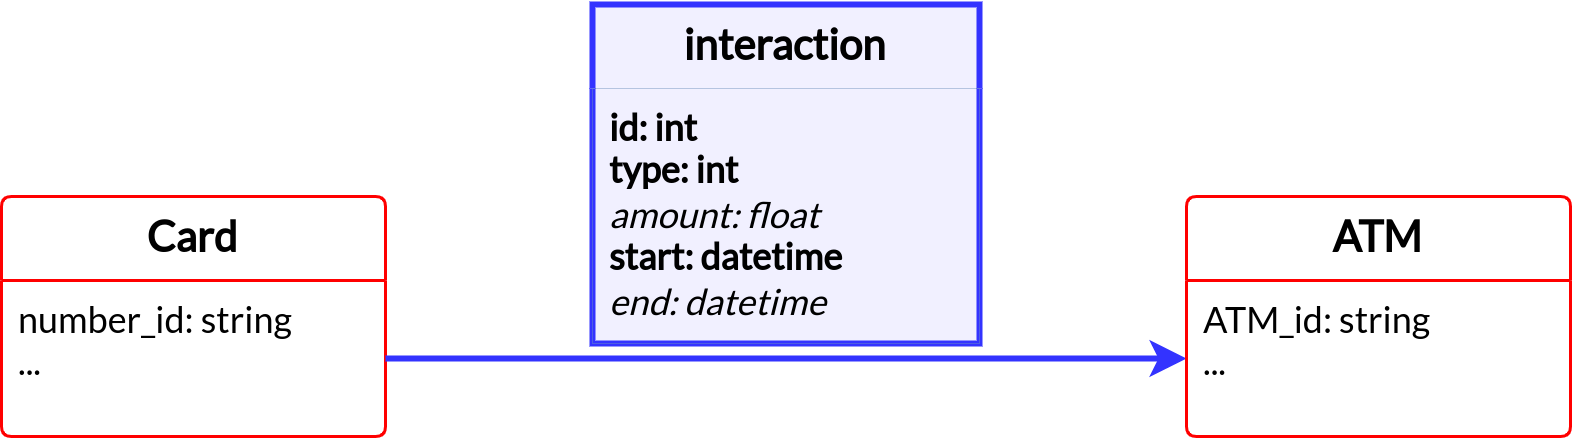
\includegraphics[scale = 0.8]{images/1-DataModel/2-edges-tx-tfm.png}
  \caption{\emph{Opening} interaction edge}
  \label{img:opening-edge}
\end{figure}

\fmc{Esto ponerlo en la definicion de interaction dentro de la definicion de volatile property graph del punto anterior}
It is important to remark that, \textcolor{gray}{as in our definition of the input data stream of the $DP_{CQE}$}, we generate two edges per transaction/\texttt{interaction} relation -- the \emph{opening} and the \emph{closing} edges -- which both will constitute a single \texttt{interaction} relation. The \emph{opening} edge (Figure \ref{img:opening-edge}) will be the indicator of the beginning of a new interaction between the matched Card and ATM, it contains the values of the properties related with the starting time \emph{start}, the interaction \emph{type} as well as the \texttt{id}. The \emph{closing} edge (Figure \ref{img:closing-edge}) will indicate the end of the interaction, completing the values of the rest of the properties of the interaction: \emph{end} and \emph{amount}.

\begin{figure}[h]
  \centering
  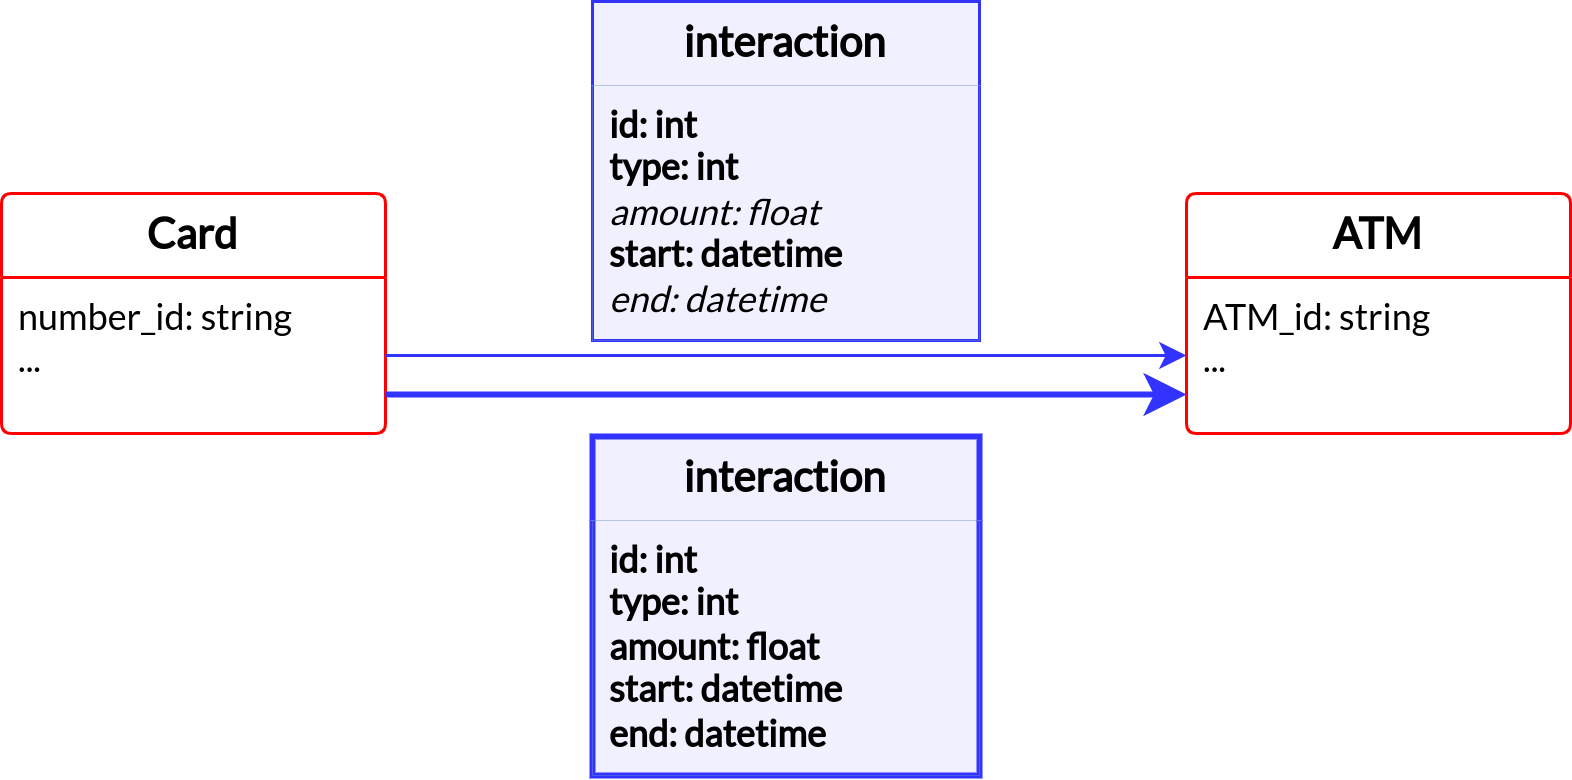
\includegraphics[scale = 0.8]{images/1-DataModel/2-edges-tx-tfm-1.png}
  \caption{\emph{Closing} interaction edge}
  \label{img:closing-edge}
\end{figure}

\textcolor{gray}{With this division of the interaction relation in two edges we are simulating that on each transaction, our system receives an initial message when the interaction starts and a final message once the interaction is finished on the ATM. Allowing us to develop a system that is able not only to detect anomalous scenarios on interactions that have already been produced/closed, but also to act in real time before the anomalous interaction detected is actually finished.}

\textcolor{red}{\rule{\linewidth}{0.5mm}}

We divide the generation of the transaction set in the generation of two subsets: the regular transaction set and the anomalous transaction set. The regular transaction set consists of the \emph{ordinary/correct} transactions, that are guaranteed to not produce any anomalous scenarios, whereas the anomalous transaction set is composed of the \emph{irregular/anomalous} transactions that are intentionally created to produce anomalous scenarios. The main reason to do this separation on the generation is to divide the creation of the full transaction stream in two steps. First the creation of the stream of the regular transaction set, having the control to ensure that no anomalous fraud scenarios are produced in between the transactions of this set. And second, and only after the creation of the regular transaction set, we create the anomalous transaction set, creating transactions that originate anomalous fraud scenarios over the regular transaction set.

\paragraph{Regular Transaction Set\\\\}

The main idea of the creation of this set, is to produce a set of ordinary transactions for each of the cards that do not produce any anomalous scenarios between them. \textcolor{gray}{Depending on the fraud types considered some constraints need to be added when doing the generation of this transaction stream in order to avoid the accidental creation of these kind of fraud patterns on this set.} After this set is created, the transactions producing anomalous scenarios related with each specific fraud pattern will be produced and injected to compose the final stream of transactions. 

\textcolor{gray}{So far, for the fraud patterns that we are considering the constraints that we need to impose on the generation of the regular transaction set are:}
\begin{enumerate}
    \renewcommand{\labelenumi}{\Roman{enumi}.} % Roman numerals for the list
    \item Fraud pattern I: No two consecutive transactions in different ATM locations can be produced with an insufficient feasible time difference.
\end{enumerate}

The transaction stream is generated for a customisable \texttt{NUM\_DAYS} number of days starting in a \texttt{START\_DATE} for each of the cards on our bank network. For each card we take its behavior (see \ref{table:behavior-properties}) to determine the number and type of interactions performed in the defined days time interval: $[\texttt{START\_DATE}, \texttt{START\_DATE} + \texttt{NUM\_DAYS}]$. The interactions are generated by linking the card to ATMs that are no farther than \texttt{MAX\_DISTANCE\_SUBSET\_THRESHOLD} kilometers from the residence location of the client of the card \texttt{residence\_loc}, given by the location coordinates of the card entity: $(loc\_latitude, loc\_longitude)$. Nevertheless, in a simpler version of the transaction generator program we also consider avoiding this limitation and allow to link the card to any ATM of the bank dataset. Finally, the interactions are distributed along the defined time interval $[\texttt{START\_DATE}, \texttt{START\_DATE} + \texttt{NUM\_DAYS}]$ respecting the constraint (I) related with the Fraud Pattern I: limit the time distance between two consecutive transactions so that, for a card, there are no two consecutive transactions in different ATM locations with an insufficient feasible time difference.

As a summary of the procedure a pseudocode of the transaction generator is depicted in Algorithm \ref{alg:regular-tx-generator}, of which some of its parts are later explained.

\fmc{TODO: Cambiar, no me gusta lo del residence\_loc, no se define así la property en la card!}
\begin{algorithm}[H]
  \small
  \begin{algorithmic}[1]
  \STATE $\texttt{id} \gets 0$
  \FOR{\text{card} in \text{cards}}
    \STATE $\texttt{ATM\_subset}, \overline{\texttt{ATM\_subset}} \gets \text{createATMsubset(\texttt{residence\_loc})}$
    \STATE $\texttt{t\_min\_subset} \gets \text{calculate\_t\_min\_subset(\texttt{ATM\_subset})}$
    \STATE $\texttt{num\_tx} \gets \text{decide\_num\_tx()}$
    \STATE $T \gets \text{distribute}(\texttt{num\_tx}, \texttt{t\_min\_subset})$
    \FOR{$t_i$ in $T$}
        \STATE $\texttt{ATM}_{i} \sim \texttt{ATM\_subset}$
        \STATE $\texttt{start}_{i} \gets t_i.start$
        \STATE $\texttt{end}_{i} \gets t_i.end$
        \STATE $\texttt{type}_{i} \gets \text{getType()}$
        \STATE $\texttt{amount}_{i} \gets \text{getAmount(}\texttt{type}_{i}\text{)}$
        \STATE $\texttt{id}_{i} \gets \texttt{id}; \ \texttt{id} \gets \texttt{id} + 1$
        \STATE $\text{createTransaction}(\texttt{id}_{i}, \texttt{ATM}_i, \texttt{start}_{i},\texttt{end}_{i}, \texttt{type}_{i}, \texttt{amount}_i)$
    \ENDFOR
    \STATE $\text{introduceAnomalous}(\texttt{ATM\_subset}, \overline{\texttt{ATM\_subset}})$ \COMMENT{Anomalous transaction set}
  \ENDFOR
  \end{algorithmic}
  \caption{Regular Transactions Generation}
  \label{alg:regular-tx-generator}
\end{algorithm}

\begin{enumerate}
    \item \textbf{Creation of the ATM subset} \\
    {\footnotesize \textcolor{teal}{$\texttt{ATM\_subset}, \overline{\texttt{ATM\_subset}} \gets \text{createATMsubset(\texttt{residence\_loc})}$}}

    \texttt{ATM\_subset} is the subset of ATMs of the stable bank dataset, in which we will allow the interactions of each of the cards to occur. We set a limit on the size of this subset, considering only a maximum ratio of the total number of ATMs on the dataset (\texttt{MAX\_SIZE\_ATM\_SUBSET\_RATIO} $\in [0,1]$), so that only a certain amount of the ATMs are included on it: 
    $$|\texttt{ATM\_subset}| = \texttt{MAX\_SIZE\_ATM\_SUBSET\_RATIO} * |\texttt{ATM}|$$ 

    There are two options for the construction of this subset:
    \begin{itemize}
        \item \textbf{Distance to cardholder residence location selection}: Only the closest $|\texttt{ATM\_subset}|$ ATMs to the cardholder residence location \texttt{residence\_loc} = \emph{(loc latitude, loc longitude)} are included in the subset. These ATMs are considered to be \textit{usual} for the cardholder, in terms of its location distance. Apart from the subset size limitation, a maximum distance constraint defined by the
        \texttt{MAX\_DISTANCE\_SUBSET\_THRESHOLD} parameter can be imposed:
        
        \begin{align*}
        \texttt{ATM\_subset} &= \{\texttt{ATM}\ |\ \texttt{distance(ATM, residence\_loc)} \\
        &\leq \texttt{MAX\_DISTANCE\_SUBSET\_THRESHOLD}\}
        \end{align*}
        
            \fmc{TODO: CAMBIAR ESTA IMAGEN}
            \begin{figure}[H]
              \centering
              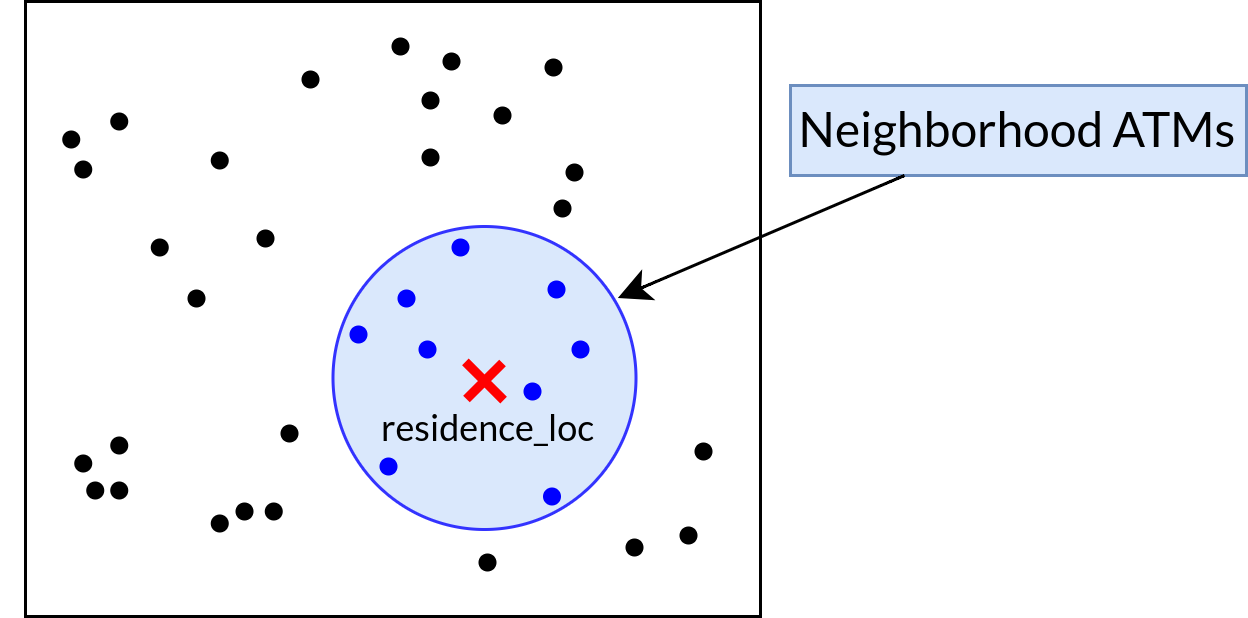
\includegraphics[scale=1.1]{images/1-DataModel/tx-generation-1-named.png}
              \caption{\texttt{Neighborhood} ATM subset}
            \end{figure}
    
        \item \textbf{Random selection}: The \texttt{ATM\_subset} is built by randomly selecting $|\texttt{ATM\_subset}|$ ATMs from the stable bank dataset.
    \end{itemize}

    \item \textbf{Calculate \texttt{t\_min\_subset}} \\
    {\footnotesize\textcolor{teal}{$\texttt{t\_min\_subset} \gets \text{calculate\_t\_min\_subset(\texttt{ATM\_subset})}$}}

    \texttt{t\_min\_subset} is the minimum threshold time needed to respect between any two consecutive transactions of a card in the regular transaction set.
    
    That is, \texttt{t\_min\_subset} is the minimum time distance between the end of a transaction and the start of the next consecutive transaction of a card, needed to guarantee in order to ensure that the constraint (I) is respected on the generation of the regular transactions set.
    
    $$\texttt{t\_min\_subset} = \frac{\texttt{max\_distance\_subset}}{\texttt{REGULAR\_SPEED}}$$

    To calculate it, we take the time needed to traverse the maximum distance between any pair of ATMs of the \texttt{ATM\_subset}: \texttt{max\_distance\_subset} at an assumed speed that any two locations can be traveled in the case of regular transaction scenarios: \texttt{REGULAR\_SPEED}.

    \item \textbf{Decide the number of transactions to be generated \texttt{num\_tx}}\\
    {\footnotesize \textcolor{teal}{$\texttt{num\_tx} \gets \text{decide\_num\_tx()}$}}
    
    Based on the behavior of the card, we decide the number of transactions \texttt{num\_tx} to generate for the card for the defined days time interval $[\texttt{START\_DATE}, \texttt{START\_DATE} + \texttt{NUM\_DAYS}]$:

    $$\texttt{num\_tx} \sim \text{Poisson}(\lambda = \texttt{ops\_day} * \texttt{NUM\_DAYS})$$ where \texttt{ops\_day} is the sum of the average number of all the kinds of operations per day of the behavior of the card: 
    $$\texttt{ops\_day} = \texttt{withdrawal\_day} + \texttt{ deposit\_day} + \texttt{ inquiry\_day} + \texttt{ transfer\_day}$$

    \item \textbf{Distribution of the \texttt{num\_tx} transaction times} \\
     {\footnotesize \textcolor{teal}{$T \gets \text{distribute}(\texttt{num\_tx}, \texttt{t\_min\_subset})$}}
    
    Along the selected time interval $[\texttt{START\_DATE}, \texttt{START\_DATE} + \texttt{NUM\_DAYS}]$ we do a random uniform distribution of the \texttt{num\_tx} transaction times. $T$ contains the list of all the the \texttt{start} and \texttt{end} times tuples for each of the \texttt{num\_tx} transactions, respecting the constraint (I) in order to guarantee that, no two consecutive transactions $tx_i$ and $tx_{i+1}$ performed in any of the ATMs of the \texttt{ATM\_subset} are at a time distance lower than \texttt{t\_min\_subset}. Specifically, the transaction times are generated guaranteeing:

    $$tx_i.\texttt{end} + \texttt{t\_min\_subset} < tx_{i+1}.\texttt{start} \ \forall i \in [1,\texttt{num\_tx})$$

    The \texttt{end} time of a transaction is assigned a shifted time difference with respect to the \texttt{start} time. In particular:

    $$
    \texttt{end} = \texttt{start} + \texttt{time\_difference}
    $$

    where:

    $$\texttt{time\_difference} \sim \mathcal{N}(\texttt{MEAN\_DURATION},\,\texttt{STD\_DURATION})$$ with the corrections:

    $$
    \texttt{time\_difference} =
    \begin{cases} 
        \texttt{MEAN\_DURATION} & \text{if } \texttt{time\_difference} < 0 \\
        \texttt{MAX\_DURATION} & \text{if } \texttt{time\_difference} > \texttt{MAX\_DURATION} \\
        \texttt{time\_difference} & \text{otherwise}
    \end{cases}
    $$

\fmc{TODO: PONER UN DIBUJITO!, explicar lo del checking de los fitting holes? --> yo creo que esto ya no es necesario... demasiado detalle}
\fmc{TODO: Explicar la variante (del generador simplificado \texttt{txGenerator-simplified.py}) en el que este distribute\_tx se cambia de tal forma que: with random order (like original version) if num holes/2 > needed holes, otherwise we introduce the transactions ordered in the time interval increasingly ordered one after
the other}

    \item \textbf{Decision on the specific values of each transaction properties:}
    Once all the previous steps are done, the specific values for the properties of each of the \texttt{num\_tx} transactions can be decided (this corresponds to the lines 7-15 in the algorithm pseudocode \ref{alg:regular-tx-generator}). Therefore for each of the transactions:
    \begin{itemize}
        \item \textbf{Link to a random ATM of the \texttt{ATM\_subset}}\\
        {\footnotesize \textcolor{teal}{$\texttt{ATM}_{i} \sim \texttt{ATM\_subset}$}}
        \item \textbf{Obtain its corresponding \emph{start} and \emph{end} time property values from the $T$ time distribution}\\
        {\footnotesize \textcolor{teal}{$\texttt{start}_{i} \gets t_i.start$, }}
        {\footnotesize \textcolor{teal}{$\texttt{end}_{i} \gets t_i.end$}}
        \item \textbf{Decide on the type of transaction}\\
        {\footnotesize \textcolor{teal}{$\texttt{type}_{i} \gets \text{getType()}$}}
        
        For each of the \texttt{num\_tx} transactions, the transaction \emph{type} is decided randomly assigning a transaction \emph{type} given a probability distribution constructed from the card behavior:
        
        $$
        \begin{cases}
          P(\texttt{type} =  \texttt{withdrawal}) = \frac{\texttt{withdrawal\_day}}{\texttt{ops\_day}} \\[8pt]
          P(\texttt{type} =  \texttt{deposit}) = \frac{\texttt{deposit\_day}}{\texttt{ops\_day}} \\[8pt]
          P(\texttt{type} = \texttt{inquiry}) = \frac{\texttt{inquiry\_day}}{\texttt{ops\_day}} \\[8pt]
          P(\texttt{type} =  \texttt{transfer}) = \frac{\texttt{transfer\_day}}{\texttt{ops\_day}} 
        \end{cases}
        $$

        where again, \texttt{ops\_day} is the sum of the average number of all the kinds of operations per day of the behavior of the card: 
        $$\texttt{ops\_day} = \texttt{withdrawal\_day} + \texttt{ deposit\_day} + \texttt{ inquiry\_day} + \texttt{ transfer\_day}$$

        \item \textbf{Assign a transaction \emph{amount}}\\
        {\footnotesize \textcolor{teal}{$\texttt{amount}_{i} \gets  \text{getAmount(}\texttt{type}_{i}\text{)}$}}
          
        The transaction \emph{amount} is assigned depending on the \emph{type} of the current transaction, based on the card behavior properties:
            
          $$
          \begin{cases}
            \mathcal{N}(\texttt{amount\_avg\_withdrawal},\, \texttt{amount\_std\_withdrawal}) & \text{if } \texttt{type} = \texttt{withdrawal} \\[10pt]
            
            \mathcal{N}(\texttt{amount\_avg\_deposit},\, \texttt{amount\_std\_deposit}) & \text{if } \texttt{type} = \texttt{deposit} \\[10pt]
        
            0 & \text{if } \texttt{type} = \texttt{inquiry} \\[10pt]
            
            \mathcal{N}(\texttt{amount\_avg\_deposit},\, \texttt{amount\_std\_transfer}) & \text{if } \texttt{type} = \texttt{transfer}
          \end{cases}
          $$
        
          $$
          \text{If } \texttt{amount} < 0, \text{ then re-draw from } U(0, 2 \cdot \texttt{amount\_avg\_type}).
          $$
        
          with \texttt{amount\_avg\_type} as \texttt{amount\_avg\_withdrawal}, \texttt{amount\_avg\_deposit} or \texttt{amount\_avg\_deposit} depending on the respective transaction \texttt{type}.   
    \end{itemize}
\end{enumerate}

An example of a transaction data item can be seen in \ref{csv:transaction}, where both the 
interaction opening and interaction close of the \emph{transaction\_id} 2804 can be observed.
\begin{center}
\lstset{style=csvStyle}
\begin{lstlisting}[caption={Example of transaction-all.csv}, label={csv:transaction}]
transaction_id,number_id,ATM_id,transaction_type,transaction_start,
transaction_end, transaction_amount
2804,c-NIGER-148,NIGER-40,0,2018-04-01 00:00:47,,
2804,c-NIGER-148,NIGER-40,0,2018-04-01 00:00:47,2018-04-01 00:04:43,26886.73
\end{lstlisting}
\end{center}

\fmc{TODO: SIGO AQUÍ!}
\textcolor{red}{\rule{\linewidth}{0.5mm}}
\fmc{TODO: Explain the simplified version of the txGenerator...:}
\textcolor{red}{For the medium size experiments (500000 cards), to generate the stream of tx, we needed to simplify this process in order to be able to generate a stream in a feasible amount of time. In particular we used the simplifed version of the \texttt{txGenerator.py}: \texttt{txGenerator-simplified.py} $\rightarrow$ with a random ATM-subset instead of a closest to client ATM-subset. Also variation on the transaction distribution times, with random order (like original version) if $num\_holes / 2 > needed\_holes$, otherwise we introduce the transactions ordered in the time interval increasingly ordered one after the other.}

\textcolor{blue}{To do the generation of the synthetic set of transactions we created the Python program \texttt{transactionGenerator.py}. On it we need to specify the value of the parameters needed to customise the generation of the set of transactions.}

\textcolor{red}{\rule{\linewidth}{0.5mm}}
\begin{itemize}
  \item Selection of ATMs:
  \begin{itemize}
    \item \textcolor{green}{$\Rightarrow$} Neighborhood / Closed ATM subset.
    \item Random walk. To do the selection of the sequence of ATMs for the generated transactions.
  \end{itemize}
  \item Distribution of the transactions along time:
  \begin{itemize}
    \item \textcolor{green}{$\Rightarrow$} Uniform distribution.
    \item \textcolor{blue}{$\Rightarrow$ (Consider the possibility)} Poisson process distribution.
  \end{itemize}
  \item Other options:
  \begin{itemize}
    \item Random walk for both the ATM and the transaction time selection, in the same algorithm together.
  \end{itemize}
\end{itemize}

\textcolor{red}{TODOS:
\begin{itemize}
\item Cambiar/Actualizar dibujos
\item Poner lista de params y explicar (tabla) como y qué se puede configurar
\item Anomalous generator:
\begin{itemize}
  \item NO-Overlapping assumption - Explain
  \item Any type of tx to produce the fraud -> does not matter the type for the FP1.
\end{itemize}
\end{itemize}
}
\textcolor{red}{\rule{\linewidth}{0.5mm}}

\paragraph{Anomalous Transaction Set\\\\}

After the generation of regular transactions we perform an injection of transactions to produce anomalous scenarios. The injection is taylored depending on the specific kind of 
anomalous scenarios that we want to produce. In what follows we explain the injection process depending on each of the types of frauds that we have considered.

\paragraph{Fraud Pattern I}

To produce anomalous scenarios related to this type of fraud, we produce the injection
of transactions that will produce the satisfaction of this fraud pattern. In other words,
we inject transactions that violate the minimum \emph{time-distance} constraint between transactions performed with the same card. Therefore, as we can see in Figure \ref{img:anomalous-type-1}, if we consider a set of regular transacions for a certain card, where $y_1$ and $y_2$ are regular consecutive transactions, we will introduce an anomalous transaction $a_{12}$ such that: 

$$(y_1.\texttt{ATM\_id} \ne a_{12}.\texttt{ATM\_id}) \land (a_{12}.\texttt{start} - 
y_1.\texttt{end} < T_{min}(y_1.\texttt{ATM\_loc}, a_{12}.\texttt{ATM\_loc}))$$

where \texttt{ATM\_loc} is the tuple of coordinates (loc\_latitude,loc\_longitude) of the corresponding ATM. This injection will produce an anomalous scenario of this kind of fraud with at least the $y_1$ previous transaction. Note that, it could possibly trigger more anomalous fraud scenarios with the subsequent transactions ($y_2$ and on...).

\begin{figure}[H]
    \centering
    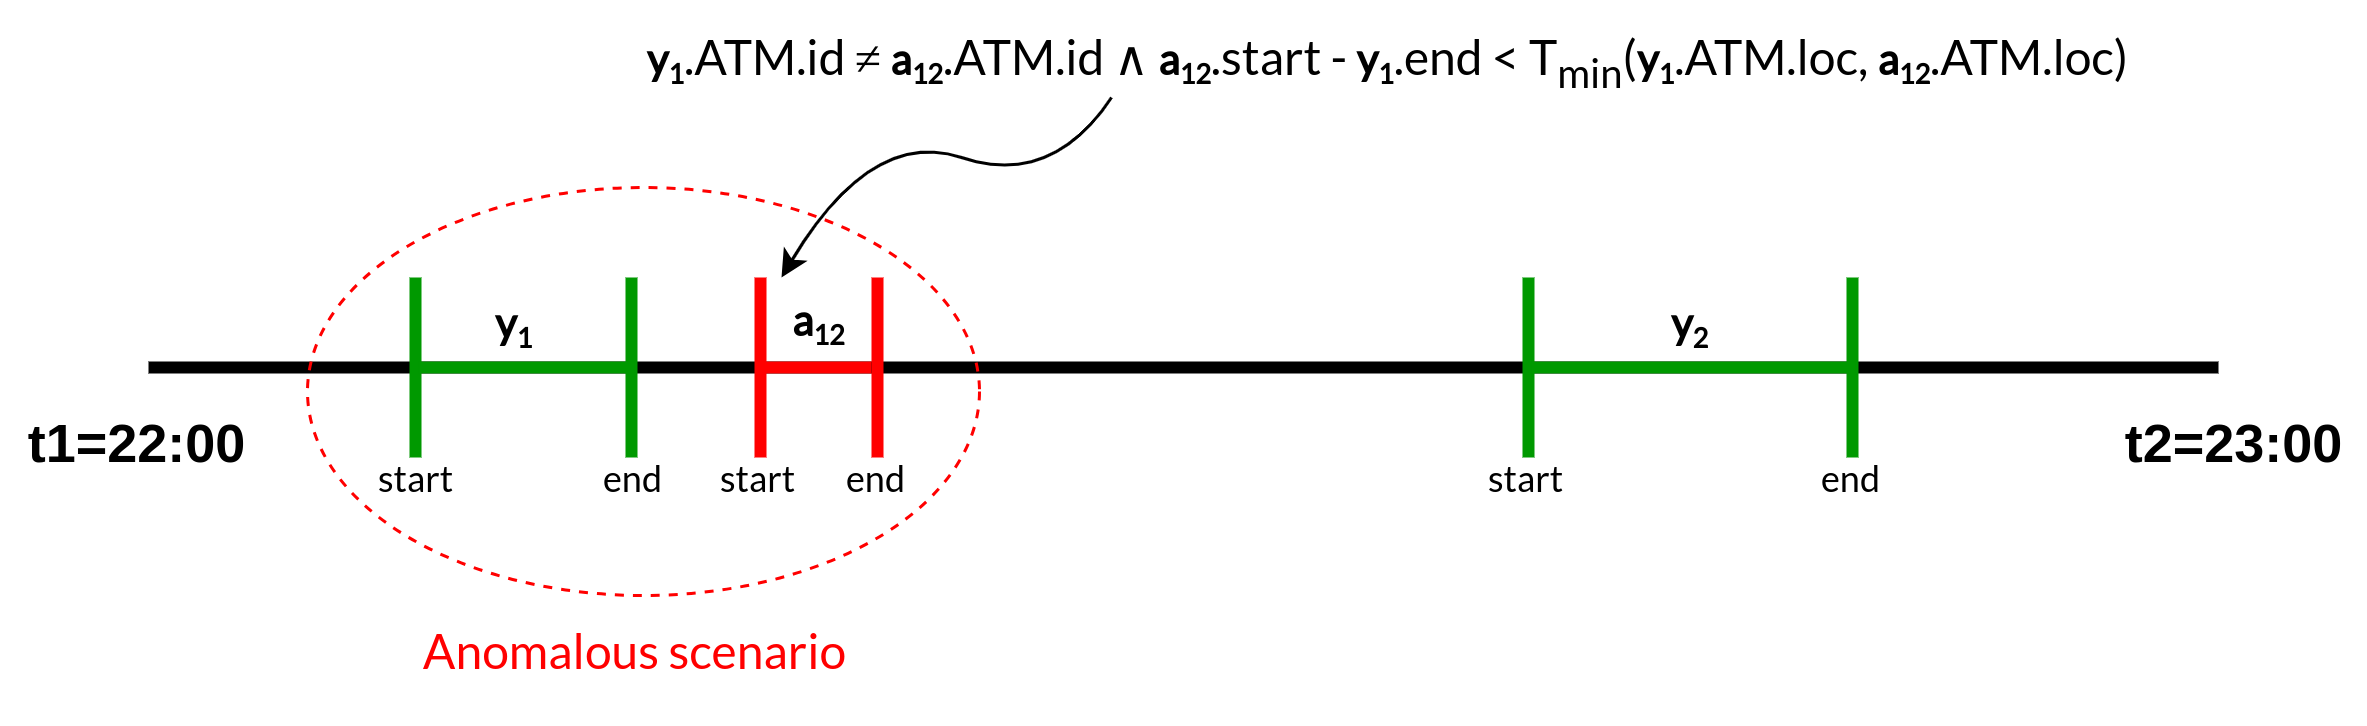
\includegraphics[width=\textwidth]{images/1-DataModel/tx-generation.png}
    \caption{Creation of anomalous scenario - type I}
    \label{img:anomalous-type-1}
\end{figure}

Some assumptions related with the generation of anomalous transactions for this kind of fraud pattern are:
\begin{itemize}
  \item \textbf{Overlapping of transactions is not possible}:
  Appart from guaranteeing that this injection causes at least one anomalous scenario, we also respect the additional constraint of ensuring that the anomalous transaction injected does not cause overlapping with any of the transactions, in particular neither with the previous nor the next one. \textcolor{orange}{This constraint is added based on the assumption that the bank itself does not allow to open a transaction whenever another one is still open.} Therefore considering that $a_{12}$ is the anomalous injected transaction in between the regular consecutive transactions $y_1$ and $y_2$, when generating $a_{12}$ we guarantee that:
  $$
  \begin{cases}
    a_{12}.\texttt{start} > y_{1}.\texttt{end} \\
    a_{12}.\texttt{end} < y_{2}.\texttt{start}
  \end{cases}
  $$
  \item \textbf{There are no two consecutive anomalous transactions}: For simplicity in our practical purposes, we do the generation of anomalous transactions for this kind of fraud pattern assuming that an anomalous transaction can only be in between two regular consecutive transactions, so that we do not consider the case of the injection of two or more consecutive anomalous transactions for this kind of fraud. See Figure \ref{img:anomalous-type-1-insertion-points}.
  \begin{figure}[H]
    \centering
    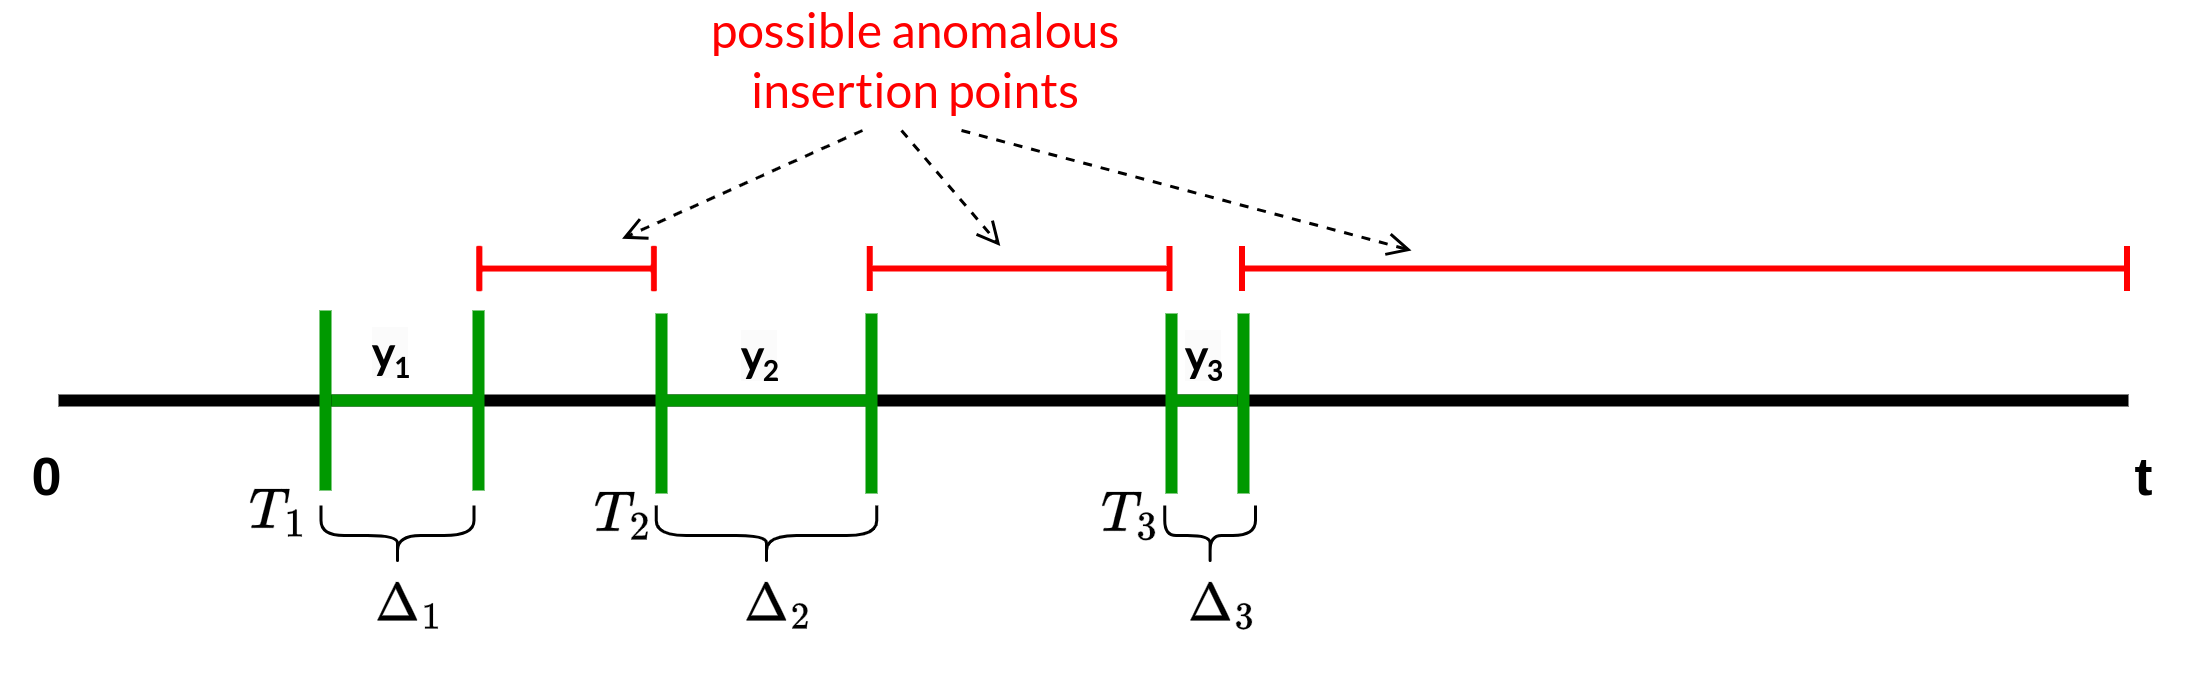
\includegraphics[width=\textwidth]{images/1-DataModel/tx-generation-anomalous-1.png}
    \caption{Considered possible injection points of anomalous transactions of fraud type I}
    \label{img:anomalous-type-1-insertion-points}
  \end{figure}  
\end{itemize}

We generate $\texttt{ANOMALOUS\_RATIO\_1} * \texttt{num\_tx}$ anomalous transactions for each of the cards related with the fraud pattern I, where $\texttt{ANOMALOUS\_RATIO\_1} \in [0,1]$ defines the ratio of anomalous transactions of this kind over the total number of regular transactions \texttt{num\_tx} for each of the cards. In Algorithm \ref{alg:anomalous-tx-generator-1} we describe at a high level the process of the generation of anomalous transactions for this kind of fraud pattern. 


\textcolor{red}{Preconditions:
\begin{itemize}
  \item ATMsubset, and the compl. are given by param, from the tx regular generator
\end{itemize}
}

\begin{algorithm}[H]
  \small
  $\textbf{introduceAnomalous}(\texttt{ATM\_subset}, \overline{\texttt{ATM\_subset}})$
  \begin{algorithmic}[1]
  \STATE $\texttt{num\_anomalous} \gets \texttt{num\_tx} * \texttt{ANOMALOUS\_RATIO\_1}$
  \STATE $i \gets 0$
  \WHILE{$i < \texttt{num\_anomalous}$}
      \STATE $\texttt{ATM}_{i} \sim \overline{\texttt{ATM\_subset}}$
      \STATE $prev_i, next_i \gets \text{randomUniquePosition(\texttt{num\_tx})}$
      \STATE $t_i \gets \text{getTime}(prev_i, next_i)$
      \STATE $\texttt{start}_{i} \gets t_i.start$
      \STATE $\texttt{end}_{i} \gets t_i.end$
      \STATE $\texttt{type}_{i} \gets \texttt{getRandomType()}$
      \STATE $\texttt{amount}_{i} \gets \texttt{getAmount()}$
      \STATE $\texttt{id}_{i} \gets \texttt{id}; \ \texttt{id} \gets \texttt{id} + 1$
      \STATE $\texttt{createTransaction}(\texttt{id}_{i}, \texttt{ATM}_i, \texttt{start}_{i},\texttt{end}_{i}, \texttt{type}_{i}, \texttt{amount}_i)$
      \STATE $i \gets i + 1$
  \ENDWHILE
  \end{algorithmic}
  \caption{Introduction of Anomalous Transactions for Fraud Pattern I}
  \label{alg:anomalous-tx-generator-1}
\end{algorithm}


\begin{enumerate}
  \item \textbf{Assignment of ATMs not belonging to the \texttt{ATM\_subset}}: the anomalous transactions are linked to ATMs that are part of the complementary of the \texttt{ATM\_subset}.
  \item \textbf{Each anomalous transaction has a unique insertion position}: As described previously, we do not allow the case of two or more consecutive anomalous transactions injection. Each anomalous transaction occupies a unique position among all the possible injection positions defined by the set of regular transactions generated for the card. As it can be seen on Figure \ref{img:anomalous-type-1-insertion-points}, considering that we have three regular transactions, we will consider three unique possible insertion points for the anomalous transactions. The procedure of assigning a unique insertion position for each anomalous transaction to be generated is achieved with the function \text{randomUniquePosition(\texttt{num\_tx})}, that given the number of regular transactions of the card \texttt{num\_tx} returns the previous and the next regular transaction to the assigned unique position.
  \item \textbf{Assign transaction times such that respecting the needed time constraints}: in particular there are two time constraints to be satisfied:
  \begin{itemize}
    \item Production of fraud pattern with prev\_i
    \item No overlapping with prev\_i nor with next\_i
  \end{itemize}
  This is summarized in the pseudocode as the procedure getTime(prev\_i, next\_i), which returns $t_i$, as the tuple of (\texttt{start},\texttt{end}) times.
  \item \textbf{Random transaction type}
  \item \textbf{Arbitrary amount}
 
\end{enumerate}

\fmc{Poner otras opciones consideradas? - ver texto comentado justo debajo}

\begin{comment}
\subsubsection{ATM closed subset + Poisson Process}

\begin{tcolorbox}
  \begin{itemize}
    \item[$\rightarrow$] \textbf{ATM selection}: Closed ATM subset.
    \item[$\rightarrow$] \textbf{Time distribution}: Poisson process distribution of $num\_tx$ 
    transactions for each of the cards.
  \end{itemize}
\end{tcolorbox}

Generate $\texttt{num\_tx}$ transactions for a selected period of time $\texttt{t}$.
Distribution following a Poisson process distribution along $[0,t]$.
\begin{itemize}
    \item[$\bullet$] $\lambda=\texttt{avg\_tx}$ on a day for the client if $\texttt{t = 24h}$. Otherwise, 
    decide a specific $\lambda$ for the considered $\texttt{t}$.
    \item[$\bullet$] Inter-arrival times $X_1, X_2, \cdots$ are distributed following an exponential distribution:
    $X_i \sim \text{Exp}(\lambda)$. They represent the time elapsed between two of these events, e.g. $X_2$ represents the time elapsed between the first and the second arrival. Note that in this case, since we need to respect the minimum required time between two consecutive 
    transactions ($t_{min}$) so to avoid introducing anomalous undesired scenarios, we have to impose
    that: $X_i \geq \Delta_{i-1} + t_{min}, \forall X_i$, where:

    \begin{itemize}
      \item[$\circ$] $X_{i}$: time elapsed between the $i$-$1$ and $i$-th transaction.
      \item[$\circ$] $\Delta_{i-1}$: time duration of the $i$-$1$ transaction. This duration will 
      be upper bounded by $\Delta_{max}$, which will be considered the maximum possible duration of a transaction.
      \item[$\circ$] $t_{min}$: minimum calculated time distance between any 2 consecutive transactions of the client.
  \end{itemize}

    With these interarrival times, we obtain the arrival times $T_i$. Note that they are not independent, in particular:
    $T_1 \leq T_2 \leq T_3 \cdots$.

    Therefore, to generate the Poisson process with rate $\lambda$:
    \begin{enumerate}
      \item Generate i.i.d. random variables $X_1, X_2, \cdots$ where $X_i \sim \text{Exp}(\lambda)$.
      \item Obtain the arrival times as:
        \begin{itemize}
          \item $T_1 = X_1$
          \item $T_2 = X_1 + X_2$
          \item $T_3 = X_1 + X_2 + X_3$
          \item $\cdots$
        \end{itemize}
    \end{enumerate}

    Note that, having imposed the previous we will have that:
    \begin{equation}
      \begin{cases}
        T_i = T_{i-1} + X_i \\
        X_i \geq \Delta_{max} + t_{min}
      \end{cases}\forall X_i \
    \end{equation}

    which implies that:
    
    \begin{equation}
      T_i \geq T_{i-1} + \Delta_{max} + t_{min}, \forall X_i
    \end{equation}
    
\end{itemize}
\begin{figure}[H]
    \centering
    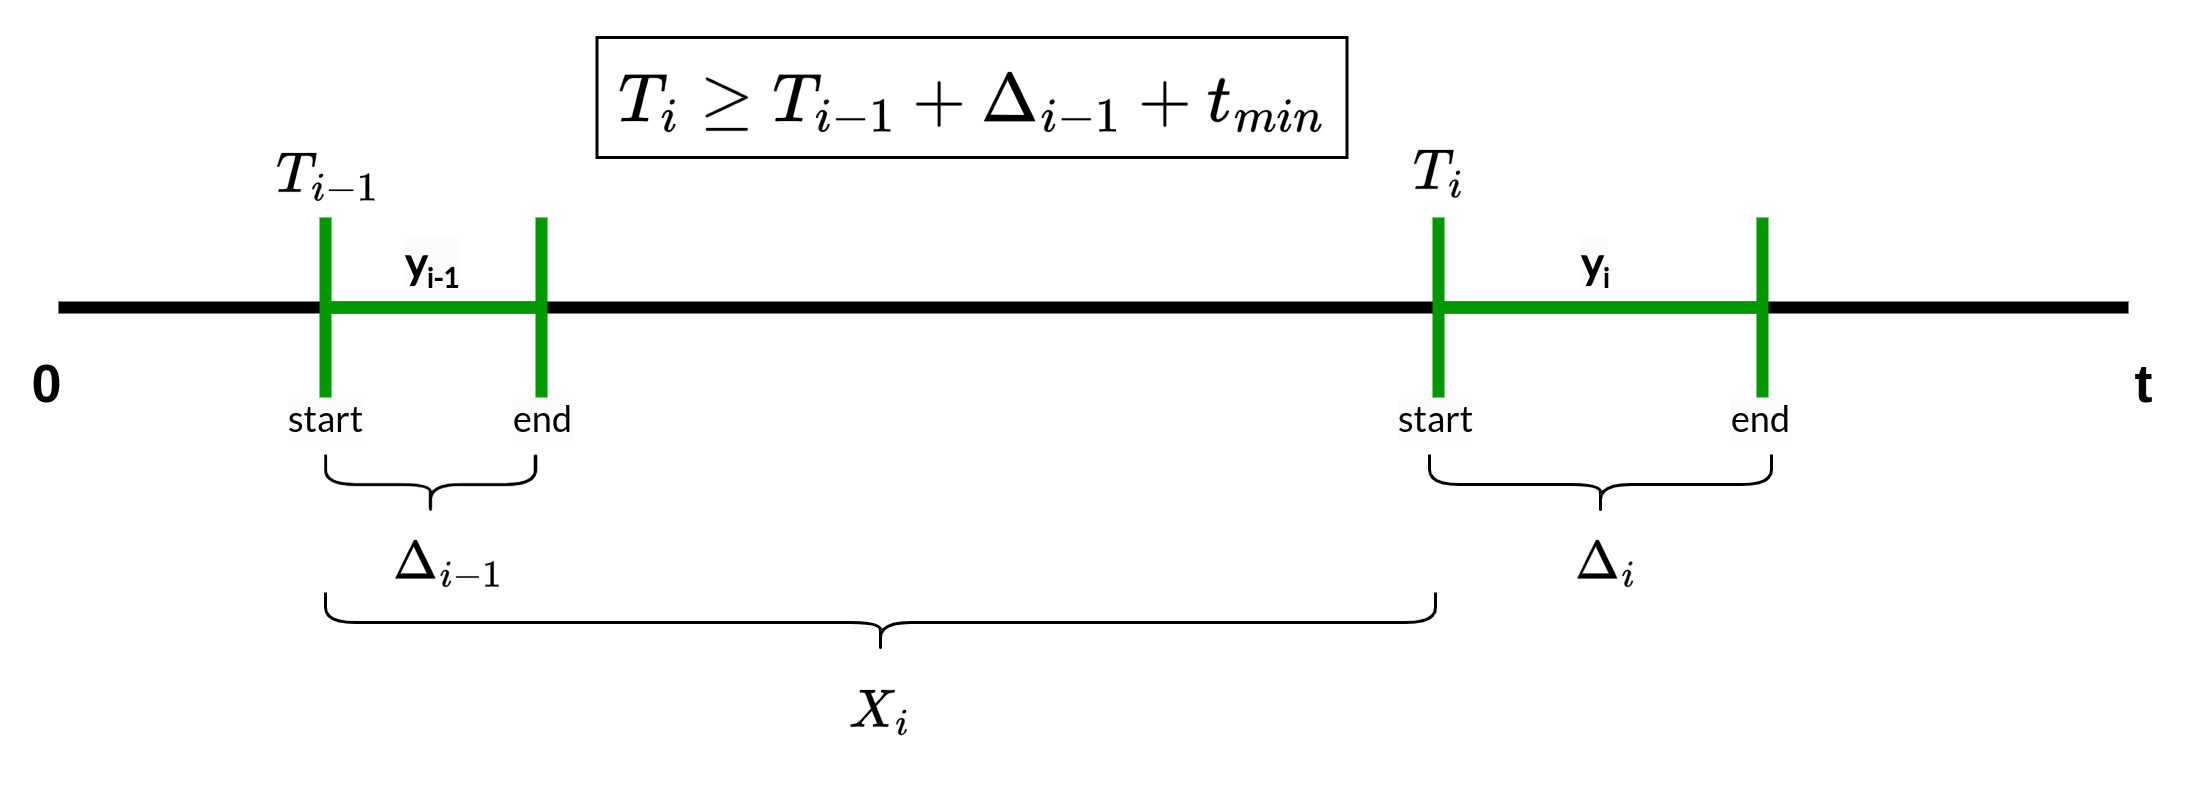
\includegraphics[scale=0.55]{images/tx-generation-dist-corrected.png}
    \caption{Schema of the interarrival and arrival event times on the poisson process.}
\end{figure}


References:

\begin{itemize}
  \item \href{https://www.probabilitycourse.com/chapter11/11_1_2_basic_concepts_of_the_poisson_process.php}{Poisson process modeling - Theoric description}
  \item \href{https://www.probabilitycourse.com/chapter14/Chapter_14.pdf}{Poisson process modeling - Python implementation}
  \item \href{https://timeseriesreasoning.com/contents/poisson-process/}{Less formal explanation with Python code}
  \item \href{https://www.math.wsu.edu/faculty/genz/416/lect/l05-45.pdf}{More theory}
  \item \href{https://en.wikipedia.org/wiki/Poisson_point_process}{Wikipedia entry}
\end{itemize}

\subsubsection{Random Walk / Markov Chain}

Idea is to model the sequence of transactions for each of the clients as a markov chain through the
network of ATMs. The network is a fully-connected graph with ATMs as nodes and edges are
weighted with the distance between each pair of ATMs as weights.

The idea is to obtain the sequence of transactions for each client as a markov chain, in which,
for each step a transaction is generated in that specific ATM node, at a certain datetime 
respecting the constraint of the minimum time distance with the previous transaction, so 
that no undesired anomalous fraud scenarios are produced. \\ 

Some considerations:
\begin{itemize}
  \item Initially, we will compute the transition matrix obtaining all the respective 
  transition probabilities. The probability of transition to another ATM-node will be 
  inversely proportional to the distance to the considered ATM-node.
  \item Transition matrix $P_t$: containing, for each state, the probability of transitioning
  between states. For example, the entry $i,j$: $(P_t)_{i,j} = \mathcal{P}(X_{t+1} = j | X_t = i)$
  contains the probability of transitioning to state $j$ when being in state $i$. 
  Note that since we assume a complete graph, and also the posibility to transition 
  to the same state, all entries of this matrix will be distinct to 0: $(P_t)_{i,j} \neq 0 \  
  \forall i,j$.
  \item Finally, once $P_t$ is computed, we perform the simulation to obtain the sequence of
  transactions for the specific card/client.
\end{itemize}

References:

\begin{itemize}
\item Markov Chains
\begin{itemize}
  \item \href{https://brilliant.org/wiki/markov-chains/}{MC - Theory}
  \item \href{https://www.columbia.edu/~ks20/4703-Sigman/4703-07-Notes-MC.pdf}{Simulation of Markov Chains - Theory}
  \item \href{https://stephens999.github.io/fiveMinuteStats/simulating_discrete_chains_1.html}{MC - Implementation example}
  \item \href{https://www.youtube.com/watch?v=G7FIQ9fXl6U}{MC - Implementation video example}
\end{itemize}
\item Random Walks
\begin{itemize}
  \item Theory:
  \begin{itemize}
    \item \href{https://ieeexplore.ieee.org/abstract/document/8911513?casa_token=vznpjKL5HG0AAAAA:hNzLCxAHBk75zCDUHsswB7ImAKgilzZcOBzxaXWz_G6U8Vy-ogbei40MoZ49M-Em5tTii0Q}{RWs: A Review of Algorithms and Applications}
    \item \href{https://www.lirmm.fr/~sau/JCALM/Josep.pdf}{RWs on Graphs}
    \item \href{https://www.fi.muni.cz/usr/gruska/random18/random1808.pdf}{RW - More theory}
  \end{itemize}
  \item Implementation examples:
  \begin{itemize}
    \item \href{https://tleise.people.amherst.edu/Math365Spring2016/RmarkdownFiles/WalkOnGraph.html}{Simple RW on a Graph - Implementation example}
    \item \href{https://graphstream-project.org/doc/Algorithms/Random-walks-on-graphs/}{A RW on a graph - Implementation}
    \item \href{https://es.mathworks.com/help/econ/simulate-random-walks-through-markov-chain.html}{Simulate Random Walks Through Markov Chain - Matlab Implementation example}
  \end{itemize}
\end{itemize}
\end{itemize}
\end{comment}

\fmc{TODO: Explain the different program versions done and how to use each. 
Files generated. Show example of the csv.}


\paragraph{Transaction dataset generator: \texttt{txGenerator.py} \\\\}

To do the generation of a transaction stream dataset we developed a Python program \texttt{txGenerator.py}. The program contains some parameters used for the customization of the generated transaction stream. 

\fmc{TODO: List the parameters to configure/set up the generation of the tx stream}
% Description/list the parameters
To use it:

\begin{enumerate}
    \item Ensure to have a \texttt{csv} named directory with the \emph{csv} stable bank dataset files on which we want to simulate a transaction stream (use the bank data generator to produce it).
    \item Run \texttt{\$> python3 txGenerator.py <outputFileName>} -- \textcolor{gray}{Run with Python3.6 version or higher} -- introducing \emph{outputFileName} as an argument to name the transaction dataset files to be generated.
\end{enumerate}

The program generates a \texttt{tx} directory with the \emph{csv} files representing the transaction stream dataset:

\begin{itemize}
    \item \texttt{<outputFileName>-all.csv}: joint regular and anomalous dataset.
    \item \texttt{<outputFileName>-regular.csv}: regular transaction dataset.
    \item \texttt{<outputFileName>-anomalous.csv}: anomalous transaction dataset.
\end{itemize}


\fmc{TODO: Explicar la versión simplificada. Random ATM subset. Actualización de la función de dsitribute\_tx, = if $num\_holes / 2 \ge needed\_holes$...}
\paragraph{Transaction dataset generator: \texttt{txGenerator-simplified.py} \\\\}

\subsection{Population of the Graph Database}

% TODO: 
% 0. Description - Neo4j, what it is, why chosen...
% 1. Creation
% 2. Population

\subsubsection{Neo4j graph database creation}
% Neo4j Desktop y version - instalación y detalles. Cómo conectarse...
% TODO: Explain how to install / connect... all the details that are in the neo4.md file
\textcolor{red}{$\rightarrow$ TODO: 0. Describe on how to set up the database}
\textcolor{red}{$\rightarrow$ TODO: Explanation of the versions of both Neo4j instances used - local and UPC VM cluster.}\\

Prior to the population of the Neo4j graph database, a Neo4j graph database instance needs to be
created. This was done both locally and in a \textcolor{red}{Virtual Machine of the UPC cluster}.

Version: Neo4j 5.21.0 Community edition. 
\begin{itemize}
    \item Accessing it: by default it runs on localhost port 7474: \texttt{http://localhost:7474}.
    Start the neo4j service locally by: \texttt{sudo systemctl start neo4j}\\
    It can be also be accessed by the internal utility \texttt{cypher-shell}. Username: \texttt{neo4j} and password: \texttt{bisaurin}.
\end{itemize}

\subsubsection{Neo4j graph database population - CSV to PG}
\begin{comment}
    - Creación de la GDB - de CSV a Neo4j PG: 
    - Poner primero los comandos cypher por separado, con las constraints de uniqueness
    y luego lo de poblar. Luego ya referir a que todo ello se tiene en un único script que 
    permite la ejecución directa (en lugar de paso a paso) en golang.
    - Incluir detalles específicos de cada CSV...
\end{comment}

Once we created the Neo4j graph database instance and all the CSV data files representing all the nodes and relations, we populate the Property Graph instance in Neo4j. Before performing the population of the GDB, we create uniqueness constraints on the properties of the nodes that we use as our \emph{de facto} IDs for the ATM and Card IDs: \texttt{ATM\_id} and \texttt{number\_id}, respectively. The reason to do this is to avoid having duplicated nodes of these types with the same ID in the database. Therefore, as an example, when adding a new ATM node that has the same \texttt{ATM\_id} as another ATM already existing in the database, we are aware of this and we do not let this insertion to happen. ID uniqueness constraints are created with the following cypher directives:

\begin{center}
\lstset{style=cypherStyle}
\begin{lstlisting}[caption={Uniqueness ID constraints}]
            CREATE CONSTRAINT ATM_id IF NOT EXISTS
            FOR (a:ATM) REQUIRE a.ATM_id IS UNIQUE
    
            CREATE CONSTRAINT number_id IF NOT EXISTS
            FOR (c:Card) REQUIRE c.number_id IS UNIQUE
    
            CREATE CONSTRAINT code IF NOT EXISTS
            FOR (b:Bank) REQUIRE b.code IS UNIQUE
\end{lstlisting}
\end{center}

Once we created the Neo4j graph database instance and all the CSV data files representing all the nodes and relations, we populate the Property Graph instance in Neo4j. For this, we propose two different methods. The first does it by directly importing the CSV files using the Cypher's \texttt{LOAD CSV} command, while the second method does it by parsing the CSV data and running the creation of the nodes and relationships using Cypher. Both methods can be found and employed using the \texttt{populatemodule} golang module.
In this module we can find the two subdirectories where each of the methods can be run. In detail, the module tree structure is depicted in Figure \ref{fig:populatemodule}. On it, the \texttt{cmd} subdirectory contains the scripts to run each of the populating methods: the first method script on \texttt{csvimport} and the second on the \texttt{cypherimport}, while the \texttt{internal} subdirectory is a library of the files with the specific functions used by these methods.

\begin{figure}[h]
\centering
\begin{forest}
  for tree={
      font=\ttfamily,              % Typewriter font for file names
      grow'=0,                      % Tree direction (left-to-right)
      child anchor=west,            % Children alignment
      parent anchor=east,           % Parent alignment
      anchor=west,                  % Tree alignment
      calign=first,                 % Aligns with the first child
      edge path={
          \noexpand\path [draw, thick, \forestoption{edge}] (!u.parent anchor) -- +(-1pt,0) |- (.child anchor)\forestoption{edge label};
      },
      inner sep=4pt,
      l=10pt,                       % Level distance
      s sep=5pt                     % Sibling distance
  }
  [populatemodule
      [cmd
        [csvimport
            [main.go]
            [.env]
        ]
        [cypherimport
            [main.go]
            [.env]
        ]
      ]
      [internal
          [common
              [common.go]
          ]
          [populate
              [populate.go]
          ]
      ]
  ]
\end{forest}
\caption{\texttt{populatemodule} file structure}
\label{fig:populatemodule}
\end{figure}

% How to run it - .env file
% Description of each of the methods


Prior to run any of these methods we need to first set up correctly the \texttt{.env} file located inside the desired method directory, where we have to define the corresponding Neo4j URI, username and password to access the Neo4j graph database instance.

\begin{itemize}
\item{\textbf{Method 1: Cypher's \texttt{LOAD CSV}}\\}
The Cypher's \texttt{LOAD CSV} clause allows to load CSV into Neo4j, creating the nodes and relations expressed on the CSV files (see \href{https://neo4j.com/docs/cypher-manual/5/clauses/load-csv/}{\textit{load-csv cypher manual}}). 
To use it simply follow these steps:
\begin{enumerate}
    \item Place all the CSVs (\texttt{atm.csv}, \texttt{bank.csv}, \texttt{card.csv}, \texttt{atm-bank-internal.csv}, \texttt{atm-bank-external.csv} 
    and \texttt{card-bank.csv}) under the \texttt{/var/lib/neo4j/import} directory
    of the machine containing the Neo4j graph database instance.
    \item Run \texttt{\$> go run populatemodule/cmd/csvimport/main.go}
\end{enumerate}

\paragraph{Process description:}

Then the different CSV files containing all the data tables of our data set, were loaded into the GDB with the following cypher directives.

% TODO: Esto es en mi local. Se recomienda por razones de seguridad... Sin embargo se puede configurar para que no sea
% así. - En el cluster veremos. De momento no pongo nada de esto!
% First, the CSV files were needed to be placed under the \texttt{/var/lib/neo4j/import} directory.

\paragraph{ATM (atm.csv)}

\begin{center}
\lstset{style=cypherStyle}
\begin{lstlisting}[caption={atm.csv}]
    LOAD CSV WITH HEADERS FROM 'file:///csv/atm.csv' AS row
    MERGE (a:ATM {
        ATM_id: row.ATM_id,
        loc_latitude: toFloat(row.loc_latitude),
        loc_longitude: toFloat(row.loc_longitude),
        city: row.city,
        country: row.country
    });
\end{lstlisting}
\end{center}

Some remarks:
\begin{itemize}
    \item \texttt{ATM} is the node label, the rest are the properties of this kind of node.
    \item Latitude and longitude are stored as float values; note that they could also be stored
    as cypher \textit{Point} data type. However for the moment it is left like this. In the future
    it could be converted when querying or directly be set as cypher point data type as property.
\end{itemize}

\paragraph{Bank (bank.csv)}

\begin{center}
\lstset{style=cypherStyle}
\begin{lstlisting}[caption={bank.csv}]
    LOAD CSV WITH HEADERS FROM 'file:///csv/bank.csv' AS row
    MERGE (b:Bank {
        name: row.name, 
        code: row.code, 
        loc_latitude: toFloat(row.loc_latitude), 
        loc_longitude: toFloat(row.loc_longitude)
    });
\end{lstlisting}
\end{center}

Note that the \texttt{code} is stored as a string and not as an integer, since to make it more clear it 
was already generated as a string code name.

\paragraph{ATM-Bank relationships (atm-bank-internal.csv and atm-bank-external.csv)}

\begin{center}
\lstset{style=cypherStyle}
\begin{lstlisting}[caption={atm-bank-internal.csv}]
    LOAD CSV WITH HEADERS FROM 'file:///csv/atm-bank-internal.csv' AS row
    MATCH (a:ATM {ATM_id: row.ATM_id})
    MATCH (b:Bank {code: row.code})
    MERGE (a)-[r:BELONGS_TO]->(b);
\end{lstlisting}
\end{center}

\begin{center}
\lstset{style=cypherStyle}
\begin{lstlisting}[caption={atm-bank-external.csv}]
    LOAD CSV WITH HEADERS FROM 'file:///csv/atm-bank-external.csv' AS row
    MATCH (a:ATM {ATM_id: row.ATM_id})
    MATCH (b:Bank {code: row.code})
    MERGE (a)-[r:INTERBANK]->(b);
\end{lstlisting}
\end{center}

\paragraph{Card (card.csv)}

\begin{center}
\lstset{style=cypherStyle}
\begin{lstlisting}[caption={card.csv}]
    LOAD CSV WITH HEADERS FROM 'file:///csv/card.csv' AS row
	MERGE (c:Card {
		number_id: row.number_id, 
		client_id: row.client_id, 
		expiration: date(row.expiration), 
		CVC: toInteger(row.CVC), 
		extract_limit: toFloat(row.extract_limit), 
		loc_latitude: toFloat(row.loc_latitude), 
		loc_longitude: toFloat(row.loc_longitude),
		amount_avg_withdrawal: toFloat(row.amount_avg_withdrawal),
		amount_std_withdrawal: toFloat(row.amount_std_withdrawal),
		withdrawal_day: toFloat(row.withdrawal_day),
		amount_avg_deposit: toFloat(row.amount_avg_deposit),
		amount_std_deposit: toFloat(row.amount_std_deposit),
		deposit_day: toFloat(row.deposit_day),
		inquiry_day: toFloat(row.inquiry_day),
		amount_avg_transfer: toFloat(row.amount_avg_transfer),
		amount_std_transfer: toFloat(row.amount_std_transfer),
		transfer_day: toFloat(row.transfer_day)
		});
\end{lstlisting}
\end{center}

Notes:
\begin{itemize}
    \item We include the fields that were generated to define the behavior of the card. They are also used for the generation of the transactions.
    \item \texttt{expiration}: set as \textit{date} data type.
\end{itemize}

\paragraph{Card-Bank relationships (card-bank.csv)}

\begin{center}
\lstset{style=cypherStyle}
\begin{lstlisting}[caption={card-bank.csv}]
    LOAD CSV WITH HEADERS FROM 'file:///csv/card-bank.csv' AS row
    MATCH (c:Card {number_id: row.number_id})
    MATCH (b:Bank {code: row.code})
    MERGE (c)-[r:ISSUED_BY]->(b);
\end{lstlisting}
\end{center}

%\subsubsection*{Dataset extensions}

\begin{comment}
- Interesting reference for coordinates and distances in cypher - https://lyonwj.com/blog/spatial-cypher-cheat-sheet 
- Transactions dataset Generation  - a transaction dataset simulator → useful with the description of fraud scenarios, that can be generated among the transactions dataset, also with customers and terminals info generation (similar to ATMs concept) 
\end{comment}

\item {\textbf{Method 2: Creation of Cypher queries\\}}

\textcolor{red}{$\rightarrow$ TODO: Describe the other population method}

\textcolor{red}{$\rightarrow$ TODO: Describe the details of the VM of the UPC cluster where the gdb is hosted -- in TFM-Neo4j/size-estimaºtion, the gmail and other files...}

\end{itemize}


\subsection{Connection to GDB}

\textcolor{red}{TODO: Add this in the data model section under a new subsection?}

Some details / notes on how this is performed in golang.


So far:
\begin{itemize}
  \item \texttt{DriverWithContext} object: only 1, shared among all the threads. It allows connections and creation of sessions. These objects are immutable, thread-safe, and fairly expensive to create, so your application should only create one instance.
  \item \texttt{Sessions}: so far we create one session every time we do a \texttt{checkFraud()} operation.
  Session creation is a lightweight operation, so sessions can be created and destroyed without significant cost. Always close sessions when you are done with them. They are not thread safe: you can share the main DriverWithContext object
  across threads, but make sure each routine creates its own sessions.
  \item \texttt{context}: context variable is not unique, and we will create one different just before needing to call functions related with the connection module.
\end{itemize}


\textcolor{blue}{\textbf{CHANGED:} 1 session per filter.\\
However, note that many multiple parallel sessions may cause overhead to the database...}
... WE ARE GOING TO ASK THE ADMIN TO KNOW THIS... In the case this is a problem we will need
to think of the pool of connections.


Some notes on this:

\begin{itemize}
  \item \href{https://neo4j.com/docs/operations-manual/current/performance/bolt-thread-pool-configuration/}{Bolt thread pool configuration}: Since each active transaction will borrow a thread from the pool until the transaction is closed, it is basically the minimum and maximum active transaction at any given time that determine the values for pool configuration options: 
  \begin{itemize}
    \item \texttt{server.bolt.thread\_pool\_min\_size}: 5 by default.
    \item \texttt{server.bolt.thread\_pool\_max\_size}: 400 by default.
  \end{itemize}
\end{itemize}

\subsection{Neo4j Details - VM Neo4j}

Tenemos una VM con Neo4j con 4 cores y 20GB de RAM.

\textcolor{red}{TODO: Add details on the Neo4j gdb and in the specific details of the VM of the UPC cluster in which we have our Neo4j gdb instance. \\
$\rightarrow$ DETAILS ON directory: "TFM/NEO4J" \href{https://github.com/FCanfran/TFM-Neo4j}{TFM-NEO4J}}

\textcolor{lightgray}{
$\rightarrow$En su día nos instalasteis una MV con Neo4j. Hemos hecho algunas pruebas y de momento bien!
Sin embargo quería preguntaros acerca de cuál es el límite en el número de sesiones que pueden haber en paralelo  (vamos a tener varios procesos en paralelo y cada uno con una sesión abierta para hacer queries a la base de datos. Estas queries en principio son todas de lectura), para entonces dependiendo de esto, saber si esto nos limita a la hora de ajustar el número de procesos que vamos a tener en paralelo.
He encontrado alguna referencia aquí:
https://neo4j.com/docs/operations-manual/current/performance/bolt-thread-pool-configuration/
donde indican que el número máximo de transacciones activas en un momento dado por defecto está en 400... No sé si esto influye en el número de sesiones o no.\\ $\rightarrow$Pues he estado buscando información y no veo en ningún sitio donde el Neo4j limite el número de sesiones que pueda haber en paralelo. Sí que he encontrado que limita el número de transacciones paralelas a 1000 por defecto, pero nada más.\\ $\rightarrow$Lo mejor es que prepares algunos tests y lo pruebes empíricamente ;)
}


\newpage

